\documentclass[review,10pt]{elsarticle}
\usepackage{amsmath,amssymb,amsthm,mathtools}
\usepackage{graphicx,booktabs,tabularx,multirow,array}
\usepackage{setspace}
\usepackage{algorithm,algpseudocode}
\usepackage{url}
\usepackage{microtype}
\usepackage{enumitem}
\usepackage{float}
\usepackage{hyperref}
\hypersetup{colorlinks=true,linkcolor=blue,citecolor=blue,urlcolor=blue}
\doublespacing
\setlength{\emergencystretch}{3em}
\newtheorem{proposition}{Proposition}
\newtheorem{theorem}{Theorem}
\newtheorem{corollary}{Corollary}
\newtheorem{remark}{Remark}
\DeclareMathOperator*{\argmin}{arg\,min}
\DeclareMathOperator{\col}{col}
\DeclareMathOperator{\rank}{rank}
\DeclareMathOperator{\spanop}{span}
\newcommand{\cX}{\mathcal X}
\newcommand{\cY}{\mathcal Y}
\newcommand{\cG}{\mathcal G}
\newcommand{\Om}{\Omega}
\newcommand{\R}{\mathbb R}
\journal{Signal Processing}
\begin{document}
\begin{frontmatter}
\title{Greedy Rank Reallocation for Budget-Constrained Tucker Tensor Completion}
\author[aff]{Angshul Majumdar\corref{cor1}}
\ead{angshul@iiitd.ac.in}
\cortext[cor1]{Corresponding author.}
\affiliation[aff]{organization={Indraprastha Institute of Information Technology Delhi (IIIT-Delhi)},city={New Delhi},country={India}}
\begin{abstract}
An incorrect Tucker multilinear rank allocation can prevent fixed-rank completion from representing the underlying tensor, even when sufficient parameters are available overall. We study a budget-aware greedy correction that removes one mode direction, adds a direction to another mode, refits the Tucker core, and accepts the exchange only after verifying the training and validation objectives. The proposed Parallel Adaptive Tucker Tensor Completion (PATT) strategy uses residual-guided candidate screening and requires no exhaustive rank search. We derive a mask-aware donor--receiver gain certificate and an inexpensive pre-refitting progress certificate, and distinguish deterministic proposal-level progress from the acceptance decision of the implemented validation-gated algorithm. Joint donor--receiver stability is established as an a priori local result, with a sharper receiver-gain bound, an executable row-wise ALS descent identity, and an explicitly conditional local refinement-basin result. A family of full-observation counterexamples shows that $h$ coupled missing mode directions can require $h$ coordinated exchanges, even when the correct rank vector is reachable through budget-feasible single exchanges. In paired CPU experiments with 25\% observed entries and deliberately incorrect ranks, PATT reaches test NMSE $\le10^{-3}$ in $2/12$, $10/12$, $10/12$, and $10/12$ trials for orders three through six, respectively. An eight-candidate Tucker rank search achieves $3/12$, $5/12$, $0/12$, and $6/12$. Correct-rank controls largely remove the advantage, and a real-data control fails the stringent threshold for all methods. Mechanism diagnostics, a new post-exchange refinement control, and a budget-detour test with more allowed greedy rounds (not lookahead) distinguish correction, local optimization, and genuine greedy stagnation. A separate certified-priority variant reduces expanded-core solves on matched one-misallocation controls, without changing the original algorithm's reported results. The contribution is corrective rank allocation, not superiority over different tensor-rank models or a global recovery guarantee.
\end{abstract}
\begin{keyword}
Tensor completion \sep Tucker decomposition \sep multilinear rank \sep greedy optimization \sep rank reallocation \sep missing data
\end{keyword}
\end{frontmatter}

\section{Introduction}\label{sec:introduction}
Low-rank models are widely used to estimate missing entries in multidimensional signal arrays. The Tucker decomposition represents a $d$-way tensor through a comparatively small core and a factor matrix in each mode. Its multilinear rank vector therefore specifies how many degrees of freedom are allocated to different signal dimensions \cite{KoldaBader2009,DeLathauwer2000svd}. When the rank vector is prescribed, the completion task reduces to nonconvex optimization over the core and factor matrices; alternating updates, multilinear spectral approximations, and geometric optimization provide well-established approaches \cite{DeLathauwer2000best,KasaiMishra2016}.

The rank vector itself can be more consequential than another round of factor optimization. A mode assigned too few directions cannot represent an essential subspace, whereas another mode may retain redundant directions. The problem is especially clear under a fixed parameter budget: merely increasing all ranks is not an option. What is needed is the ability to \emph{revise an earlier allocation decision}. We study a simple donor--receiver operation that removes one basis direction from one mode and adds one to another, preserving the allowed Tucker parameter count. The changes are evaluated using the actual observed-entry least-squares objective, not a surrogate rank score.

Rank adaptation for tensors is not new. TMac performs parallel factorizations of mode unfoldings and includes adaptive rank strategies \cite{XuHaoYinSu2015}; rank-adaptive Tucker completion based on alternating matrix completion and singular-value thresholding was proposed in \cite{LiuShiLiao2023}. More recently, geometric methods for Tucker rank varieties have provided gradient-based rank-adaptive optimization \cite{GaoPengYuan2025}, while an adaptive rank-estimation framework for image completion uses backtracking and pseudo-observations \cite{MiHeLiLiu2026}. Our contribution is narrower: we consider the \emph{explicit, budget-constrained transfer of rank between Tucker modes} after a local fit, with parallelizable candidate generation and a safeguard against increasing training error. We do not assert that the method discovers the optimal rank vector or supersedes those prior algorithms.

Tensor models based on CP, tensor train, tubal, or unfolding ranks are also meaningful, but their rank parameters are not interchangeable with Tucker multilinear ranks \cite{KoldaBader2009,LiuMusialskiWonkaYe2013}. Consequently, the central comparisons in this work use Tucker-based optimizers and identical observation sets. Source-guided Python implementations of other published methods are reported separately and are not represented as original-code executions.

Our specific contributions are as follows. First, we formulate rank exchange using the \emph{exact} Tucker parameter budget, including the core interaction term and the limitations of the reachable rank graph. Second, we describe a practical correction step based on donor truncation, residual-derived receiver directions, shortlisting, and safeguarded local refinement. Third, we derive a computable pre-refitting sufficient-progress certificate alongside the exact mask-aware gain bound, and establish a priori local donor--receiver stability and exact descent for the row-wise Tucker ALS routine without equating proposal progress with validation acceptance. We also characterize fixed-rank error floors, exchange-graph reachability, and a general $h$-mode residual-invisibility obstruction that prevents any strictly improving one-swap scheme from making progress until all coupled deficient modes are repaired. Fourth, we provide paired experiments, correct-rank controls, a limited rank-search comparison, and negative results, with NMSE $10^{-3}$ as the target accuracy rather than an incentive to optimize below the required level.

\section{Problem formulation}\label{sec:problem}
Let $\cY\in\R^{n_1\times\cdots\times n_d}$ denote the incomplete signal tensor, $d\geq 3$, and let $\Om$ be its set of observed indices. We use $\mathcal P_{\Om}$ for the sampling operator and seek a reconstruction
 \(\cX=\cG\times_1 U_1\times_2\cdots\times_d U_d, \quad U_k\in\R^{n_k\times r_k},\quad U_k^\top U_k=I.\) 
The core is $\cG\in\R^{r_1\times\cdots\times r_d}$, with multilinear rank allocation $\boldsymbol r=(r_1,\dots,r_d)$ and $1\leq r_k\leq n_k$. Define the observed-data objective
\begin{equation}\label{eq:objective}
F(\cX)=\frac12\|\mathcal P_{\Om}(\cY-\cX)\|_F^2.
\end{equation}
The stored parameter count is
\begin{equation}\label{eq:budget}
P(\boldsymbol r)=\sum_{k=1}^{d}n_kr_k+\prod_{k=1}^{d}r_k.
\end{equation}
We minimize \eqref{eq:objective} over Tucker tensors satisfying $P(\boldsymbol r)\leq B$. The budget in \eqref{eq:budget} is a representation count rather than the dimension of the quotient manifold; using it to compare candidate updates keeps the constraint meaningful for an actual stored model.

For fixed factor matrices $\boldsymbol U=(U_1,\ldots,U_d)$, the core is determined by a linear least-squares problem. If $m=|\Om|$, $y\in\R^m$ collects observed values and $\Phi_{\boldsymbol U}\in\R^{m\times R}$ denotes the sampled Kronecker-feature design, $R=\prod_k r_k$, then
\begin{equation}\label{eq:corels}
\widehat g(\boldsymbol U)\in\argmin_{g\in\R^R}\frac12\|y-\Phi_{\boldsymbol U}g\|_2^2,
\qquad \Phi_{\boldsymbol U}(\omega,:)=\bigotimes_{k=1}^d U_k(\omega_k,:),
\end{equation}
where a consistent Kronecker ordering is used throughout. Pseudoinverse least squares provides a well-defined minimum-residual solution even if the sampled features are rank deficient. We write $f(\boldsymbol U)$ for the optimal value of \eqref{eq:corels}.

The train/validation/test split is distinct from the mathematical objective. Only training entries are used to construct candidates and fit the core. Validation entries decide whether a candidate is accepted and when to stop; test entries are evaluated only after the run. In the numerical study, the target is independent-test NMSE $\leq10^{-3}$. This \emph{testing criterion} is not substituted into the training loss during optimization.

\section{Greedy correction of Tucker rank allocations}\label{sec:method}
\subsection{A rank exchange has a nontrivial cost}\label{subsec:exchange}
Choose distinct donor and receiver modes $i$ and $j$. The proposed ranks satisfy $r'_i=r_i-1$, $r'_j=r_j+1$, and $r'_k=r_k$ otherwise. Let $Q_{ij}=\prod_{k\neq i,j}r_k$. Direct substitution into \eqref{eq:budget} gives
\begin{equation}\label{eq:budgetdifference}
\begin{split}
P(\boldsymbol r')-P(\boldsymbol r)
&=n_j-n_i+\big[(r_i-1)(r_j+1)-r_ir_j\big]Q_{ij}\\
&=n_j-n_i+(r_i-r_j-1)Q_{ij}.
\end{split}
\end{equation}
An exchange is admissible if $r_i\ge2$, $r_j<n_j$ and $P(\boldsymbol r')\le B$. Unlike a simple conservation rule on $\sum_k r_k$, equation \eqref{eq:budgetdifference} accounts for the change in the Tucker core size. The full cost is always recomputed when screening candidates.

\subsection{Donor pruning and residual-guided receiver expansion}\label{subsec:construct}
After a few fixed-rank ALS sweeps, we possess current orthonormal factors and a fitted core. For donor mode $i$, compute an SVD of the mode-$i$ core unfolding. Its left singular vectors rotate the donor basis without changing the represented tensor; the last rotated direction is then deleted. This chooses a low-core-energy direction for removal. Core energy is a heuristic for the donor choice, \emph{not} an exact measure of its loss on the sampling mask. The pruned factors are therefore refitted against the observed entries before proceeding.

Let $\boldsymbol U^{-i}$ denote the pruned factors, $\cX^{-i}$ their fitted reconstruction, and $e_\omega=\cY_\omega-\cX^{-i}_\omega$ its training residual. To add one receiver direction, form a residual-weighted mode-$j$ matrix
\begin{equation}\label{eq:receiver}
H_j=\sum_{\omega\in\Om} e_\omega\, e_{\omega_j}
\left(\bigotimes_{k\neq j} U_k^{-i}(\omega_k,:)\right),
\end{equation}
where $e_{\omega_j}$ is a coordinate vector in $\R^{n_j}$ and $H_j$ has $n_j$ rows. The leading left singular vector of $(I-U_j^{-i}U_j^{-i\top})H_j$ supplies a candidate direction orthogonal to the retained receiver subspace. When the matrix vanishes, that candidate is skipped. The proposed factor is formed by adjoining the normalized vector to $U_j^{-i}$.

Every admissible donor--receiver pair is screened by solving \eqref{eq:corels} for the candidate factors. The lowest-loss few candidates are given a small number of ALS sweeps, after which the core is refitted. An exchange is accepted only if its observed training objective has not increased and its validation error has strictly improved. This check prevents a screening approximation from silently increasing the fitting objective. It does not guarantee an improvement on unseen test entries.

The evaluated implementation uses a short list of candidates, at most two rank-exchange rounds, and serial execution for the reported CPU experiments. The donor--receiver screens do not depend on one another and can in principle be evaluated on separate workers. We do not report an empirical parallel speedup for the final implementation.

\subsection{Safeguarded greedy algorithm}\label{subsec:algorithm}
\begin{algorithm}[tbp]
\caption{PATT: budget-aware greedy Tucker rank exchange}\label{alg:patt}
\begin{algorithmic}[1]
\Require Training entries $(y,\Om)$, validation set $V$, factors $\boldsymbol U_0$, budget $B$, number of exchange rounds $T$, shortlist size $s$, tolerance $\eta\ge0$.
\State Run initial fixed-rank Tucker ALS; refit the core by \eqref{eq:corels}.
\For{$t=0,1,\ldots,T-1$}
 \State Record current training loss $F_t$ and validation loss $V_t$.
 \For{each ordered donor--receiver pair $(i,j)$, $i\neq j$}
  \State Reject if $r_i\le1$, $r_j\ge n_j$, or \eqref{eq:budgetdifference} violates $B$.
  \State Rotate and prune mode $i$; refit the reduced core.
  \State Build a receiver direction using \eqref{eq:receiver}.
  \State Refit the proposed core and record its training loss.
 \EndFor
 \State Sort feasible proposals by training loss; retain at most $s$.
 \State Apply a short ALS refinement and core refit to each retained proposal.
 \State Among proposals with training loss $\le F_t-\eta$ and validation loss $<V_t$, choose the lowest-validation-loss one.
 \If{no proposal satisfies both checks}
  \State \textbf{break}
 \EndIf
 \State Accept the chosen proposal and its rank vector.
\EndFor
\State \Return final factors, core, ranks, validation history and elapsed time.
\end{algorithmic}
\end{algorithm}

The pseudocode allows $\eta=0$ (nonincreasing training loss). For a strict finite-step acceptance guarantee we use $\eta>0$. The actual experiments use a small numerical tolerance and a fixed maximum number of exchange rounds; neither choice requires theorems about global tensor recovery.

\section{Analysis: why a rank exchange can work}\label{sec:analysis}
The results distinguish \emph{allocated factor dimensions} from exact multilinear rank. A model with $r_k$ factor columns only guarantees $\operatorname{rank}(\cX_{(k)})\leq r_k$. Its actual rank also satisfies $\operatorname{rank}(\cX_{(k)})\leq\prod_{\ell\ne k}r_\ell$; equality requires a full-row-rank mode-$k$ core unfolding. All proposed exchanges preserve an upper-rank budget; exact rank recovery is asserted only under the nondegeneracy assumptions made below.

\subsection{Feasibility and limitations of single-unit exchanges}\label{subsec:feasibility}
\begin{proposition}[Feasibility and rank-sum invariant]\label{prop:budget}
If $P(\boldsymbol r_0)\leq B$ and every proposed move $\boldsymbol r'=\boldsymbol r-\boldsymbol e_i+\boldsymbol e_j$ satisfies $r_i\ge2$, $r_j<n_j$, and $P(\boldsymbol r')\le B$, then all iterates respect the allocated-rank and parameter budgets. However, every such sequence preserves $\sum_k r_k$; feasible rank allocations need not be connected by these moves.
\end{proposition}
\begin{proof}
Removing and adding orthonormal basis columns preserves the Tucker factor constraints. Equation~\eqref{eq:budgetdifference} calculates the exact budget change, proving feasibility by induction. Summing the coordinates of $-\boldsymbol e_i+\boldsymbol e_j$ gives zero, proving invariance. To establish that the graph may be disconnected even when rank sums match, take mode dimensions $(4,5,6)$, $B=94$, initial ranks $(3,2,6)$ and target $(4,5,2)$. Their parameter counts are $94$ and $93$, and both rank sums equal $11$. Exhausting the feasible ordered single-unit moves from the initial vector gives only $(4,1,6)$, with parameter count $81$; from $(4,1,6)$ the only feasible move returns to $(3,2,6)$. Thus the target is in another component.\end{proof}

The invariant can be removed by budget-feasible rank births, deaths, or multi-unit transfers. More fundamentally, \emph{reachability is not sufficient for progress}: even connected correct ranks can be inaccessible to strictly decreasing single exchanges, as the following result demonstrates. These extended moves are not part of the main experimental implementation.


\subsection{A fundamental multi-mode obstruction}\label{subsec:obstruction}
\begin{theorem}[An $h$-mode obstruction and its block-spectral escape]\label{thm:hmode}
For every $h\ge2$, let $d=2h$, $n_k=3$, and let $0<|a|\le1$. Consider
\begin{equation}\label{eq:hmodel}
\cY^\star=e_1^{\otimes 2h}+a\,e_2^{\otimes h}\otimes e_1^{\otimes h}.
\end{equation}
The true allocated ranks can be $(2,\ldots,2,1,\ldots,1)$ with $h$ twos, while the initial allocation is $(1,\ldots,1,2,\ldots,2)$ with $h$ ones followed by $h$ twos. Equip the deficient modes with the factor $e_1$ and surplus modes with $\operatorname{span}\{e_1,e_3\}$. Then both allocations, and every intermediate allocation obtained by transferring one rank unit from each of $t$ surplus modes to distinct deficient modes, $0\le t\le h$, use the same budget $B=9h+2^h$. Under full observation the optimal loss at every $t<h$ is $a^2/2$, while it is zero at $t=h$. Thus no strictly improving single-transfer algorithm starting at the stated factors can make the first move, although an $h$-transfer feasible path exists. Conversely, the residual of the initial exact fit, contracted against $e_1$ in the last $h$ modes, is the rank-one $h$-way tensor $a\,e_2^{\otimes h}$: its mode-unfolding leading singular vectors recover all $h$ missing directions simultaneously, and the coordinated $h$-transfer block proposal exactly reconstructs $\cY^\star$.
\end{theorem}
\begin{proof}
All rank allocations described above have rank sum $3h$ and core dimension $2^h$, hence budget $3(3h)+2^h$. If $t<h$, at least one of the first $h$ modes has allocated dimension one. Its true unfolding has orthogonal singular components of sizes $1$ and $|a|$; its best rank-one approximation retains error $a^2$. Therefore any Tucker reconstruction with that allocation has loss at least $a^2/2$. The original tensor $e_1^{\otimes 2h}$ remains representable after every indicated redundant-donor deletion and has precisely that loss, proving the bound is attained at all $t<h$. Once all $h$ transfers are made, the resulting factor product contains both summands of~\eqref{eq:hmodel}, so its core fit is exact. Finally, contraction against the last $h$ correct factors cancels neither component, but the residual after fitting the first term contains only $a e_2^{\otimes h}$; each of its $h$ unfoldings has a unique nonzero left singular vector $e_2$. This constructs the simultaneous block receiver directions.\end{proof}

Theorem~\ref{thm:hmode} does not say that a practical block search identifies the correct subset of $h$ receiving modes at low cost. It proves only that this coordinated correction is sufficient in the stated identifiable model and that a positive-improvement-only single-exchange algorithm cannot replicate it. No block-lookahead implementation is included in the primary PATT experiments.

\subsection{The fixed-rank error floor}\label{subsec:floor}
\begin{proposition}[Unavoidable approximation error of an underspecified mode]\label{prop:floor}
Let $\cY^\star$ be the complete noiseless tensor, and let $\cX$ have allocated mode-$i$ rank at most $r_i$. Then
\begin{equation}\label{eq:tailfloor}
\|\cX-\cY^\star\|_F^2\ge\sum_{\ell>r_i}\sigma_\ell^2(\cY^\star_{(i)}).
\end{equation}
The same lower bound divided by $\|\cY^\star\|_F^2$ applies to full-tensor NMSE, regardless of the number of fixed-rank ALS sweeps.
\end{proposition}
\begin{proof}
The mode-$i$ unfolding of $\cX$ has matrix rank at most $r_i$. Unfolding preserves Frobenius norm, so Eckart--Young--Mirsky applied to $\cY^\star_{(i)}$ proves~\eqref{eq:tailfloor}.\end{proof}

Equation~\eqref{eq:tailfloor} is a \emph{full-tensor} lower bound; it is not automatically a bound on a particular training or test mask. If a sampling operator obeys $\|\mathcal P_\Omega(\cY^\star-\cX)\|_F^2\ge p(1-\delta)\|\cY^\star-\cX\|_F^2$ on the pertinent reconstruction differences, it yields the corresponding sampled-error floor after multiplication by $p(1-\delta)$. Such restricted conditioning cannot hold uniformly for every low-rank tensor when some entries are entirely unobserved.

\subsection{The exact gain and a computable exchange certificate}\label{subsec:gain}
Let $A_0$ be the sampled full-core design of the incumbent after an \emph{exact} least-squares core fit, and let $F_0=f(A_0)$ with $f(A)=\frac12\min_x\|y-Ax\|_2^2$. For donor mode $i$, rotate the factor $U_i$ by the left singular vectors of the mode-$i$ core unfolding and delete its last column. Let $\sigma_i$ be that unfolding's smallest singular value, $A$ the resulting reduced sampled design, and $e=(I-P_A)y$ the residual after \emph{refitting} the reduced core. Write $L_i=f(A)-F_0$ for the deletion cost. The receiver mode is $j\ne i$; after pruning its factor $V=U_j$ still has $r_j$ orthonormal columns. Let $q=\prod_{k\ne j}r_k^{-i}$, and let $H_j\in\R^{n_j\times q}$ be the residual contraction in~\eqref{eq:receiver} using the pruned factors. Define $H_j^\perp=(I-VV^\top)H_j$ and $s_{ij}=\|H_j^\perp\|_2$.

For a unit receiver direction $v\perp\operatorname{col}(V)$, let $Z(v)\in\R^{m\times q}$ be the sampled design for the newly added row of core coefficients. Let $W(v)=(I-P_A)Z(v)$ and $b(v)=Z(v)^\top e=H_j^\top v$. Full-grid orthonormality of the remaining factors implies $Z(v)^\top Z(v)\preceq I_q$, even though the sampled feature Gram need not be isotropic.

\begin{proposition}[Exact receiver gain and donor loss]\label{prop:gain}
The optimally refitted receiver gain for a fixed $v$ is
\begin{equation}\label{eq:exactgain}
G(v)=f(A)-f([A\ Z(v)])=\tfrac12 b(v)^\top[W(v)^\top W(v)]^\dagger b(v).
\end{equation}
Moreover, $0\le L_i\le\sigma_i^2/2$ and $G(v)\ge\|H_j^\top v\|_2^2/2$.
\end{proposition}
\begin{proof}
Because $\operatorname{col}([A,Z])=\operatorname{col}(A)\oplus\operatorname{col}((I-P_A)Z)$, the Pythagorean identity for least-squares projections yields~\eqref{eq:exactgain}. For the donor bound, the truncated unrefitted core differs from the incumbent by a full-grid tensor with Frobenius norm $\sigma_i$, because all factors are orthonormal and the deleted core component is the last SVD slice. Since the incumbent core fit is exactly least squares, its sampled residual is orthogonal to every sampled column of $A_0$, including this deleted component. Thus the loss of the unrefitted truncation is exactly one half of the squared \emph{sampled} deletion norm, at most $\sigma_i^2/2$. Refitting in $A$ cannot increase this cost. Finally, $0\preceq W(v)^\top W(v)\preceq Z(v)^\top Z(v)\preceq I_q$. Since $b(v)\in\operatorname{range}(W(v)^\top)$, its pseudoinverse quadratic form is at least $\|b(v)\|_2^2$, which proves the receiver bound.\end{proof}


\begin{theorem}[SVD donor selection under a sampled subspace embedding]\label{thm:donoroptimal}
Let $\widehat\cX$ have an exactly refitted core $\widehat\cG$ and fixed orthonormal factors, and suppose the sampling operator on its \emph{entire fixed Tucker product subspace} satisfies
\begin{equation}\label{eq:donoriso}
p(1-\delta_0)\|Z\|_F^2\le\|\mathcal P_\Omega Z\|_F^2\le p(1+\delta_0)\|Z\|_F^2,
\quad0\le\delta_0<1.
\end{equation}
For a unit donor direction $v$ in mode-$i$ factor coordinates, let $\ell_i(v)$ denote the training-loss increase after deleting $v$ and optimally refitting all retained core coefficients. Then
 \(\frac{p(1-\delta_0)}2\|v^\top\widehat G_{(i)}\|_2^2 \le\ell_i(v)\le \frac{p(1+\delta_0)}2\|v^\top\widehat G_{(i)}\|_2^2.\) 
Consequently, for $v_{\rm svd}$, a smallest left singular vector of $\widehat G_{(i)}$,
\begin{equation}\label{eq:donorapprox}
\ell_i(v_{\rm svd})\le\frac{1+\delta_0}{1-\delta_0}
\min_{\|v\|=1}\ell_i(v).
\end{equation}
\end{theorem}
\begin{proof}
The sampled least-squares residual of the full incumbent is orthogonal to every column of its sampled product design. For any pruned factor subspace $\mathcal S_v$ of the full product space, Pythagoras gives $\ell_i(v)=\tfrac12\min_{Z\in\mathcal S_v}\|\mathcal P_\Omega(\widehat\cX-Z)\|_F^2$. Apply~\eqref{eq:donoriso} to each difference $\widehat\cX-Z$. The full-grid minimum is $\tfrac12\|v^\top\widehat G_{(i)}\|_2^2$ because the Tucker factors are orthonormal. The smallest left singular vector minimizes this quantity. Applying the two inequalities to it and to a minimizing actual donor proves~\eqref{eq:donorapprox}.\end{proof}

Theorem~\ref{thm:donoroptimal} is a guarantee for the \emph{donor step}, not for the jointly best donor--receiver exchange. The fixed-subspace embedding can be inspected through sampled Gram eigenvalues. Matrix concentration for a factor basis estimated using the same entries does \emph{not} follow merely by treating that basis as fixed.


\begin{theorem}[Mask-aware certified greedy rank-exchange improvement]\label{thm:certificate}
Fix an admissible donor--receiver pair, let $\ell_i$ be the \emph{actual} optimally refitted donor deletion cost, and let $v$ be an eligible unit receiver direction. Set $b(v)=H_j^\top v$, $W(v)=(I-P_A)Z(v)$, and $\Lambda(v)=\lambda_{\max}(W(v)^\top W(v))$. Whenever $\Lambda(v)>0$, the exact core-refitted candidate satisfies
\begin{equation}\label{eq:certgain}
\boxed{\;F_0-F(\cX_{ij}(v))\ge
\frac{\|b(v)\|_2^2}{2\Lambda(v)}-\ell_i.\;}
\end{equation}
When $\Lambda(v)=0$, the gain is zero. In particular, if $\Lambda(v)\le p(1+\delta_R)$, the leading residual-SVD direction gives
 \(F_0-F(\cX_{ij})\ge \frac{s_{ij}^2}{2p(1+\delta_R)}-\ell_i.\) 
Without any embedding assumption, $\Lambda(v)\le1$ and $\ell_i\le\sigma_i^2/2$, recovering the coarser valid bound $\tfrac12(s_{ij}^2-\sigma_i^2)$.
\end{theorem}
\begin{proof}
By Proposition~\ref{prop:gain}, $G(v)=\tfrac12 b(v)^\top(W^\top W)^\dagger b(v)$. Since $b(v)$ lies in the range of $W^\top$, the nonzero eigenvalues of $(W^\top W)^\dagger$ are at least $1/\Lambda(v)$; hence $G(v)\ge\|b(v)\|^2/(2\Lambda(v))$. Subtract the exact donor loss $\ell_i$. The normalized sampling and full-grid versions follow from the stated upper bounds on the feature Gram. If $\Lambda(v)=0$ then $W=0$, $b=0$, and the enlarged model has no additional sampled span.\end{proof}

The mask-aware certificate requires only the observed design and actual donor deletion loss, both computed during screening. It is a training-loss statement: validation rejection may still produce a zero accepted improvement. A spectral candidate can also improve with a negative certificate, since the certificate is a lower bound.



\begin{theorem}[Pre-refitting sufficient-progress certificate]\label{thm:prefit}
Assume the incumbent core has been exactly refitted. Rotate the donor factor so that its last column corresponds to the smallest singular direction of the core unfolding, and let $d_i\in\R^m$ be the \emph{sampled fitted contribution} of the core slice deleted by raw truncation. Let $r_0=y-\widehat y_0$ be the incumbent sampled residual. For a budget-feasible receiver direction $v\perp U_j$, form its $m\times q$ sampled new-feature matrix $Z_i(v)$ using the retained donor factors, without first refitting the pruned core. Put
 \(b_i(v)=Z_i(v)^\top(r_0+d_i),\qquad \lambda_i(v)=\lambda_{\max}(Z_i(v)^\top Z_i(v)).\) 
Then the exact least-squares refit in the enlarged Tucker product satisfies, whenever $\lambda_i(v)>0$,
\begin{equation}\label{eq:prefitcert}
\boxed{\;F_0-F_{ij}(v)\ge
 \frac{\|b_i(v)\|_2^2}{2\lambda_i(v)}
 -\frac{\|d_i\|_2^2}{2}
 \ge \frac{\|b_i(v)\|_2^2-\|d_i\|_2^2}{2}.\;}
\end{equation}
If $\lambda_i(v)=0$, the bound is $-\|d_i\|_2^2/2$. Writing
$H_{j,\rm raw}^{\perp}$ for the projected residual contraction of $r_0+d_i$ against the retained nonreceiver factors, its leading left singular vector maximizes $\|b_i(v)\|_2$. Therefore the computable condition
\begin{equation}\label{eq:prefitpositive}
\sigma_1^2(H_{j,\rm raw}^{\perp})>\|d_i\|_2^2+2\eta
\end{equation}
certifies a training improvement of at least $\eta$ \emph{before any new core refit}. The condition is sufficient, not necessary; failure of~\eqref{eq:prefitpositive} does not justify safely discarding a candidate that might improve after refitting.
\end{theorem}
\begin{proof}
Since the incumbent is least-squares fitted, $r_0$ is orthogonal to its sampled design, including the deleted contribution $d_i$. Raw truncation therefore has residual $r_0+d_i$ and increases training loss by precisely $\|d_i\|^2/2$. Adding an arbitrary new-feature coefficient $c$ without changing the retained old coefficients gives residual $r_0+d_i-Z_i(v)c$. The enlarged exact refit cannot have greater loss than the minimum over this restricted family. The least-squares gain in this restricted family is $b_i(v)^\top[Z_i(v)^\top Z_i(v)]^\dagger b_i(v)/2$. Since $b_i(v)$ belongs to the Gram matrix range, this is at least $\|b_i(v)\|^2/[2\lambda_i(v)]$. The full-grid columns underlying $Z_i(v)$ are orthonormal, so $Z_i(v)^\top Z_i(v)\preceq I$ and $\lambda_i(v)\le1$. Finally, the usual contraction identity gives $b_i(v)=H_{j,\rm raw}^{\top}v$; maximizing its norm over $v\perp U_j$ yields the leading singular vector and~\eqref{eq:prefitpositive}.\end{proof}

This certificate needs the current core slice, the sampled residual, and a sparse contraction; it does \emph{not} need an intermediate donor-core refit, receiver Gram inversion, or expanded-core least squares. It can be used to prioritize guaranteed-improving proposals before expensive refits. A nonpositive lower bound is inconclusive and cannot be used for a lossless pruning rule. The original benchmark implementation did \emph{not} employ this new pre-refitting prioritization; a dedicated numerical check is reported in Section~\ref{subsec:mechanism}.


\begin{theorem}[Certified gain for the receiver actually used by PATT]\label{thm:actualreceiver}
Let the incumbent core be exactly refitted on the training mask. After deleting its selected donor slice, let $r_{\rm raw}=r_0+d_i$ and let $A$ be the sampled reduced-core design. The donor-refitted residual used by Algorithm~\ref{alg:patt} is
\begin{equation}\label{eq:rawrefit}
r_-= (I-P_A)r_{\rm raw}=r_{\rm raw}-P_A d_i,
\end{equation}
since $r_0\perp\operatorname{col}(A)$. Let $H_{\rm raw}^{\perp}$ and $H_-^{\perp}$ be the receiver contractions of these two residuals, projected orthogonally to the current receiver factor. Put
$\epsilon_H=\|H_{\rm raw}^{\perp}-H_-^{\perp}\|_2$. If $v_-$ is the leading left singular vector of $H_-^{\perp}$, the \emph{same direction selected by the implemented residual-SVD screening}, then
\begin{equation}\label{eq:bridge}
\|H_{\rm raw}^{\perp\top}v_-\|_2
\ge [\sigma_1(H_{\rm raw}^{\perp})-2\epsilon_H]_+,
\qquad \epsilon_H\le\|P_A d_i\|_2,
\end{equation}
where the second inequality assumes distinct sampled entries, as in the experiments. In particular, if $\ell_i=f(A)-F_0$ is the \emph{actual refitted donor loss}, the enlarged model after exact core fitting satisfies the directly computable, \emph{pre-expansion} guarantee
\begin{equation}\label{eq:postdonorcert}
\boxed{F_0-F_{ij}(v_-)\ge\tfrac12\sigma_1^2(H_-^{\perp})-\ell_i.}
\end{equation}
The alternative raw-residual certificate for this very direction is
\begin{equation}\label{eq:bridgecert}
F_0-F_{ij}(v_-)\ge\tfrac12[\sigma_1(H_{\rm raw}^{\perp})-2\epsilon_H]_+^2-\tfrac12\|d_i\|_2^2.
\end{equation}
Both bounds apply to the \emph{unrefined} exact-core-fit proposal generated by Algorithm~\ref{alg:patt}; neither by itself ensures validation acceptance.
\end{theorem}
\begin{proof}
The reduced design is a subspace of the initial sampled product design, so the exactly fitted incumbent residual $r_0$ is orthogonal to it. Hence~\eqref{eq:rawrefit}. The residual-contraction map is the composition of zero insertion at distinct sampled coordinates, mode unfolding, multiplication by an orthonormal Kronecker factor, and projection on the receiver complement; each has operator norm at most one from sampled Euclidean norm to matrix Frobenius norm. Thus $\epsilon_H\le\|P_A d_i\|_2$. By the triangle inequality and optimality of $v_-$ for $H_-^{\perp}$,
$\|H_{\rm raw}^{\perp\top}v_-\|\ge\sigma_1(H_-^{\perp})-\epsilon_H\ge\sigma_1(H_{\rm raw}^{\perp})-2\epsilon_H$.
For the actual post-pruning residual, Proposition~\ref{prop:gain} and the sampled Gram upper bound $W^\top W\preceq I$ give receiver gain at least $\frac12\|H_-^{\perp\top}v_-\|^2=\frac12\sigma_1^2(H_-^{\perp})$. Subtracting $\ell_i$ proves~\eqref{eq:postdonorcert}. Applying Theorem~\ref{thm:prefit} to $v_-$ and the first inequality of~\eqref{eq:bridge} proves~\eqref{eq:bridgecert}.
\end{proof}

Theorem~\ref{thm:actualreceiver} removes the receiver-direction discrepancy between Theorem~\ref{thm:prefit} and the evaluated algorithm. Computing~\eqref{eq:postdonorcert} after the already-performed donor core fit and residual SVD does not require the expanded-core least-squares solve. The benchmark version still executes that solve for screening, so the theorem supplies a verifiable \emph{screening priority}, not a measured runtime saving or a guarantee that a negative certificate permits candidate rejection.

\subsection{When the spectral direction approximates the best receiver}\label{subsec:screenquality}
Under arbitrary masks, the residual SVD maximizes $\|b(v)\|_2$, not the exact gain~\eqref{eq:exactgain}. The following result quantifies the distinction.
\begin{theorem}[Restricted-conditioning approximation ratio]\label{thm:ratio}
Suppose for the fixed pruned model that every eligible unit receiver vector $v$ satisfies
\begin{equation}\label{eq:gramcond}
\mu I_q\preceq W(v)^\top W(v)\preceq L I_q,
\qquad0<\mu\le L.
\end{equation}
Then the spectral receiver $v_{ij}$ obeys
\begin{equation}\label{eq:ratio}
G(v_{ij})\ge\frac{\mu}{L}\max_{\|v\|=1,\,v\perp V}G(v).
\end{equation}
If the full-grid subspace $\mathcal K_j=\R^{n_j}\otimes\bigotimes_{k\ne j}\operatorname{col}(U_k^{-i})$ satisfies
\begin{equation}\label{eq:embedding}
(1-\delta)p\|z\|_2^2\le\|\mathcal P_\Omega K_jz\|_2^2\le(1+\delta)p\|z\|_2^2
\end{equation}
for every $z$, where $K_j$ is an orthonormal basis of $\mathcal K_j$, then~\eqref{eq:gramcond} holds with $\mu=p(1-\delta)$ and $L=p(1+\delta)$, giving ratio $(1-\delta)/(1+\delta)$.
\end{theorem}
\begin{proof}
By~\eqref{eq:exactgain} and~\eqref{eq:gramcond}, $\|b(v)\|^2/(2L)\le G(v)\le\|b(v)\|^2/(2\mu)$. The spectral receiver maximizes the middle score $\|b(v)\|^2$, giving~\eqref{eq:ratio}. For the second claim, full-grid old and newly added feature columns are orthonormal and lie in $\mathcal K_j$. Thus for any $z$, $\|W(v)z\|^2=\min_x\|A x+Z(v)z\|^2$. Apply~\eqref{eq:embedding} to the joint subspace and use $\|A_{\mathrm{full}}x+Z_{\mathrm{full}}z\|^2=\|x\|^2+\|z\|^2$. Minimizing the lower bound and choosing $x=0$ in the upper bound proves the asserted Gram inequalities.\end{proof}

The subspace embedding in~\eqref{eq:embedding} is \emph{uniform over receiver directions}, including a direction computed adaptively from the training mask. It is not asserted for arbitrary tensors. For a fixed $K_j\in\R^{N\times q_K}$ with $q_K=n_j\prod_{k\ne j}r_k^{-i}$ and coherence $\mu_K=(N/q_K)\max_\omega\|(K_j)_{\omega,:}\|_2^2$, independent Bernoulli-$p$ observation gives~\eqref{eq:embedding} with probability at least $1-\alpha$ when, for instance,
\begin{equation}\label{eq:chernoff}
pN\ge\frac{8\mu_Kq_K}{\delta^2}\log\frac{2q_K}{\alpha},\qquad0<\delta<1.
\end{equation}
This follows from matrix Chernoff concentration~\cite{Tropp2012}; the constant 8 is conservative. For Kronecker Tucker factors, $\mu_K=\prod_{k\ne j}\mu(U_k^{-i})$, where $\mu(U_k)=(n_k/r_k)\max_a\|U_k(a,:)\|^2$. Thus bounded factor incoherence and sufficient random observations give an explicit approximation factor. Structured block masks can violate~\eqref{eq:embedding} even when factor coherence is small. The matrix-Chernoff statement requires $K_j$ to be fixed independently of the mask (for instance, ideal nonreceiver subspaces or factors estimated from an independent pilot set). It cannot be applied without further analysis to nonreceiver factors learned adaptively from the same observations.

\begin{table}[tbp]
\caption{The sufficient fixed-subspace sample-size criterion~\eqref{eq:chernoff} does \emph{not} cover any primary configuration. The minimum shown uses the optimistically best coherence $\mu_K=1$, $\alpha=.05$, and the limiting choice $\delta\uparrow1$, whereas the theorem requires $\delta<1$. This is not a claim that the actual sampled Gram matrices are singular.}\label{tab:samplegap}
\centering\small
\begin{tabular}{crrr}
\toprule
Order & Available training $m$ & Dimension $q_K$ & Optimistic sufficient $m$\\
\midrule
3 & 672 & 56 & 3,456\\
4 & 2,970 & 88 & 5,750\\
5 & 6,048 & 128 & 8,746\\
6 & 11,025 & 224 & 16,309\\
\bottomrule
\end{tabular}
\end{table}



\subsection{Limits of donor--receiver screening}\label{subsec:pairquality}
Theorem~\ref{thm:ratio} compares receiver directions \emph{for a fixed donor}. Theorem~\ref{thm:donoroptimal} compares donor deletion costs. These separate approximation factors do not multiply into a universal approximation ratio for the jointly optimal exchange: a donor with small deletion cost need not have the best receiver gain. An additive bound involving an unrestricted donor loss can be nonpositive, making it uninformative. We therefore do not claim a global approximation ratio over all feasible donor--receiver pairs. Instead, the positive-progress theorem below identifies a concrete one-swap correction regime in which the actual screened candidate is guaranteed to lower the objective by a strictly positive quantity.


\subsection{Exact one-swap correction and incomplete-sampling stability}\label{subsec:oneswap}
\begin{theorem}[Exact correction of one misplaced Tucker rank]\label{thm:exactrecovery}
Let $\cY^\star$ be noiseless with exact Tucker ranks $\boldsymbol r^\star$. Suppose all observed entries are available, and the incumbent allocated ranks equal $\boldsymbol r^\star+\boldsymbol e_i-\boldsymbol e_j$ for distinct modes $i,j$. Assume: (i) the donor factor contains the true mode-$i$ subspace plus exactly one orthogonal redundant column; (ii) the receiver factor $V$ spans a codimension-one subspace of the true mode-$j$ subspace; (iii) every other mode factor spans its true subspace; (iv) the incumbent fitted mode-$i$ core unfolding has rank $r_i^\star$ (hence its only null left singular direction is precisely the redundant donor direction), and both core fits are exact; and (v) the proposed exchange is budget feasible. Then $\sigma_i=0$, and for some $a\ne0$ and unit $u_\perp\perp V$ the pruned residual contraction satisfies
\begin{equation}\label{eq:rankoneH}
H_j=u_\perp a^\top.
\end{equation}
The leading receiver singular vector is $\pm u_\perp$, and the subsequent Tucker core refit exactly reconstructs $\cY^\star$ in one exchange. Its resulting allocated dimensions equal $\boldsymbol r^\star$, and its exact multilinear ranks equal $\boldsymbol r^\star$.
\end{theorem}
\begin{proof}
Let $K_{-j}=\bigotimes_{k\ne j}U_k^\star$. Since the donor factor contains the true donor space and every other nonreceiver factor is correct, there exists $C\in\R^{n_j\times q}$ with $\cY^\star_{(j)}=C K_{-j}^\top$, and $\operatorname{col}(C)$ equals the true mode-$j$ subspace. With $V$ of codimension one therein, decompose $C=VB+u_\perp a^\top$, $a\ne0$. The full-data least-squares incumbent equals the orthogonal projection onto its factor product subspace, namely $VB K_{-j}^\top$, and has no core energy in the surplus donor direction: hence $\sigma_i=0$. Assumption (iv) ensures the smallest-singular-vector truncation removes that redundant direction rather than a different zero-energy true direction. Donor deletion leaves the fit unchanged. The residual unfolding is $u_\perp a^\top K_{-j}^\top$; contracting it against $K_{-j}$ gives~\eqref{eq:rankoneH}. Its unique nonzero left singular direction is $u_\perp$. Adding this direction restores the entire true product subspace, so the exact core refit has zero error. Because the true tensor has exact Tucker ranks $\boldsymbol r^\star$, the enlarged fitted core must have full corresponding unfolding ranks.\end{proof}

The full-observation theorem is a local structural recovery statement, not global rank identifiability or a guarantee from arbitrary initialization. The following quantitative perturbation result covers a restricted incomplete-observation setting without assuming that the rank-one signal alone determines all possible missing entries.


\begin{theorem}[Joint donor--receiver stability under incomplete observations]\label{thm:stability}
Assume the donor and receiver containment geometry of Theorem~\ref{thm:exactrecovery}, but allow all other mode factors to deviate from their true subspaces by principal angles $\epsilon_k=\|(I-U_kU_k^\top)U_k^\star\|_2$ for $k\notin\{i,j\}$. Set $\eta=\sum_{k\notin\{i,j\}}\epsilon_k$. The incumbent factor subspaces are held fixed during the core fit; their full-data orthogonal-projection core is $G^0$, with a one-dimensional left nullspace at donor mode $i$ and smallest nonzero singular value
 \(\gamma_i=\sigma_{r_i-1}(G^0_{(i)})>0.\) 
Let $S$ be the sampling restriction, $p=|\Omega|/N$, and let the observed data be $y=S\operatorname{vec}(\cY^\star)+\xi$, $\|\xi\|_2\le\nu$. The incumbent sampled design $A_0=S\Phi_0$ obeys $\|p^{-1}A_0^\top A_0-I\|_2\le\delta_0<1$. Define $X^0=\Pi_0\cY^\star$ and
 \(\varepsilon_G= \frac{\|p^{-1}A_0^\top[S\operatorname{vec}(\cY^\star-X^0)+\xi]\|_2}{1-\delta_0}, \qquad a_i=\min\{1,2\varepsilon_G/\gamma_i\}.\) 
Let $\widehat v_i$ be the smallest left singular vector of the \emph{sampled fitted} core; delete it, then refit the pruned core using $S$. Let $\mathcal S^-$ be the ideal pruned product space, $\widehat{\mathcal S}^-$ its estimated counterpart, $X^{0,-}=\Pi^-\cY^\star$, and $\widehat X^-$ the sampled pruned refit. Assume the sampled design $\widehat A^-$ for $\widehat{\mathcal S}^-$ satisfies $\|p^{-1}(\widehat A^-)^\top\widehat A^--I\|_2\le\delta_-<1$. Define
 \(\varepsilon_-=\frac{\|p^{-1}(\widehat A^-)^\top[S\operatorname{vec}(\cY^\star-\widehat\Pi^-\cY^\star)+\xi]\|_2}{1-\delta_-}\); \(d_-=a_i\|\cY^\star\|_F+\varepsilon_-.\) 
Align the pruned-factor bases by an orthogonal change of core coordinates. If $K_0$ and $\widehat K$ are the ideal and estimated Kronecker products of the nonreceiver factors, let $E_0=\cY^\star-X^{0,-}$, $e_0=\|E_0\|_F$, and let $s=\|(I-VV^\top)(E_0)_{(j)}K_0\|_2>0$. Because the receiver subspace is nested in its true subspace with codimension one, this contracted matrix is rank one with nonzero singular value $s$ (even when other factors are slightly inaccurate). Set
 \(\tau_D=\sup_{0\neq D\in\mathcal S^-+\widehat{\mathcal S}^-} \frac{\|SD\|_2}{p\|D\|_F}\); \(\zeta_s=\|[\{(p^{-1}S^\top S-I)\operatorname{vec}(E_0)\}_{(j)}]\widehat K\|_2\); \(\nu_H=\|[p^{-1}S^\top\xi]_{(j)}\widehat K\|_2\); \(\zeta=\zeta_s+\sqrt2\,a_i e_0+\tau_D d_-+\nu_H.\) 
Here $[\cdot]_{(j)}$ means reshape as a mode-$j$ unfolding. The normalized projected residual used to select the new receiver is $\widehat H_j^\perp=(I-VV^\top)[p^{-1}S^\top(y-S\widehat X^-)]_{(j)}\widehat K$. Then the actual deleted donor direction has angle at most $a_i$ to the ideal redundant direction, and
\begin{equation}\label{eq:jointreceiver}
\|\widehat H_j^\perp-u_\perp c^\top\|_2\le\zeta,
\quad \sin\angle(\widehat u_j,u_\perp)\le
 b_j:=\min\{1,\zeta/(s-\zeta)\},\qquad \zeta<s,
\end{equation}
where $\widehat u_j$ is its leading left singular direction and $\|c\|=s$. Finally, if the sampling operator obeys a $(1\pm\delta_+)$ embedding on the sum of the ideal true product space and the \emph{actual} enlarged product space, the final sampled core-refitted reconstruction satisfies
\begin{equation}\label{eq:jointreconstruction}
\boxed{\quad
\|\widehat\cX-\cY^\star\|_F
\le \sqrt{\frac{1+\delta_+}{1-\delta_+}}
(a_i+b_j+\eta)\|\cY^\star\|_F
+\frac{2\nu}{\sqrt{p(1-\delta_+)}}.\quad}
\end{equation}
\end{theorem}
\begin{proof}
Write the ideal full-grid incumbent as $X^0=\Phi_0g^0$. The sampled normal equations give $\widehat g-g^0=(A_0^\top A_0)^{-1}A_0^\top[S(\cY^\star-X^0)+\xi]$, whence $\|\widehat G-G^0\|_F\le\varepsilon_G$. Because $G^0_{(i)}$ has one zero singular value separated by $\gamma_i$, $\sigma_{\min}(\widehat G_{(i)})\le\varepsilon_G$. If $\widehat v_i$ is the corresponding left singular vector, then $\|G^{0\top}_{(i)}\widehat v_i\|\le2\varepsilon_G$. On the orthogonal complement of the ideal null direction the smallest singular value is $\gamma_i$; therefore $\sin\angle(\widehat v_i,v_i^0)\le 2\varepsilon_G/\gamma_i$. The pruned donor projectors consequently differ by at most $a_i$.

The second sampled normal equation gives $\|\widehat X^--\widehat\Pi^-\cY^\star\|_F\le\varepsilon_-$. Multilinear projection and the donor projector bound imply $\|\widehat\Pi^-\cY^\star-\Pi^-\cY^\star\|_F\le a_i\|\cY^\star\|_F$; hence $\|\widehat X^--X^{0,-}\|_F\le d_-$. After alignment, the nonreceiver product factors satisfy $\|\widehat K-K_0\|_2\le\sqrt2 a_i$ (a principal-angle/Procrustes inequality). Expand the normalized sampled receiver residual around $E_0$, adding and subtracting $(E_0)_{(j)}\widehat K$. The four resulting errors are sampling of $E_0$ (at most $\zeta_s$), changing $K_0$ to $\widehat K$ (at most $\sqrt2 a_i e_0$), replacing $X^{0,-}$ with $\widehat X^-$ (at most $\tau_Dd_-$), and measurement noise (at most $\nu_H$). Left projection by $I-VV^\top$ does not enlarge their norms, proving the first inequality in~\eqref{eq:jointreceiver}. Since the ideal contraction is $u_\perp c^\top$ of rank one and singular value $s$, the leading singular value of the perturbed contraction is at least $s-\zeta$. Projecting its leading singular-vector equation orthogonally to $u_\perp$ gives the angular bound in~\eqref{eq:jointreceiver}.

Projecting the true tensor onto the retained nonreceiver mode subspaces creates an approximation error at most $\eta\|\cY^\star\|_F$ by telescoping orthogonal mode projections. Correct donor deletion and adjoining $u_\perp$ represent this projection; perturbing the donor and receiver projectors by at most $a_i,b_j$ therefore yields a candidate full-grid approximation error no greater than $(a_i+b_j+\eta)\|\cY^\star\|_F$. Optimal sampled least squares on the actual enlarged product cannot have a larger sampled residual than this approximation, apart from twice the observation-noise norm. Apply the assumed sampling embedding to both residual differences to obtain~\eqref{eq:jointreconstruction}.\end{proof}

Theorem~\ref{thm:stability} treats \emph{both} the donor SVD and the receiver residual and allows nonzero principal-angle errors in other modes, rather than assuming successful donor deletion or fully correct remaining factors. The parameters $\delta_0,\delta_-,\delta_+,\tau_D,\zeta_s$ are geometric conditions on the \emph{actual} sampled subspaces and errors. A sufficient fixed-subspace matrix-Chernoff sample size cannot be applied automatically to training-adaptive factors. This theorem is therefore a deterministic local stability statement, not a proof that the sample sizes in Table~\ref{tab:instances} satisfy a uniform random-mask theorem.


\begin{theorem}[Off-signal rather than bulk residual perturbation]\label{thm:offsig}
In an ideal local one-swap configuration, suppose the projected receiver contraction has rank one, $H_\star=sua^\top$, with $s>0$ and $\|u\|=\|a\|=1$. Write the actual normalized sampled contraction as $\widehat H=H_\star+E$ and define
 \(w=\widehat H^\top u, E_\perp=(I-uu^\top)E\); \(A_u=\|w\|_2^2, D_u=\|E_\perp\|_2^2\); \(B_u=\|E_\perp w\|_2.\) 
If $A_u>D_u$, the leading left singular vector $\widehat u$ of $\widehat H$ obeys
 \(\tan\angle(\widehat u,u)\le\frac{B_u}{A_u-D_u}.\) 
In particular, perturbation parallel to $u$ does not rotate the recovered direction. This is an \emph{a priori/oracle} bound: $u$, and thus $E_\perp$, is unknown during completion. It is not an observed-data certification rule.
\end{theorem}
\begin{proof}
Decompose $\widehat H\widehat H^\top$ in the orthogonal splitting $\operatorname{span}(u)\oplus u^\perp$. Its upper-left block is $A_u$, its off-diagonal block has norm $B_u$, and its bottom-right positive-semidefinite block has norm at most $D_u$. The largest eigenvalue $\lambda$ is at least $A_u>D_u$; hence its unit eigenvector has a nonzero $u$ component $\alpha$ and complementary component $z$. The complementary eigen-equation gives
$\|z\|\le B_u|\alpha|/(\lambda-D_u)\le B_u|\alpha|/(A_u-D_u)$.
Since $\tan\angle(\widehat u,u)=\|z\|/|\alpha|$, the claimed inequality follows.
\end{proof}

\begin{theorem}[Off-signal stability implies one-swap training progress]\label{thm:targetprogress}
For the exact receiver chosen by Algorithm~\ref{alg:patt}, use the normalized post-donor residual contraction $\widehat H=p^{-1}H_-^\perp$ and the ideal unit direction $u$ from Theorem~\ref{thm:offsig}. Let $A_u=\|\widehat H^\top u\|_2^2$, $D_u=\|(I-uu^\top)\widehat H\|_2^2$, and $B_u=\|(I-uu^\top)\widehat H\,\widehat H^\top u\|_2$. For the actual selected direction $v_-$, let $\Lambda=\lambda_{\max}(W(v_-)^\top W(v_-))>0$ and let $\ell_i$ be the exactly refitted donor deletion loss. Then the exact expanded-core refit satisfies
\begin{equation}\label{eq:targetgain}
\boxed{F_0-F_{ij}(v_-)\ge \frac{p^2 A_u}{2\Lambda}-\ell_i.}
\end{equation}
This lower bound does \emph{not} require the bulk condition $\zeta<s$ in Theorem~\ref{thm:stability}, nor does it require $A_u>D_u$. If $A_u>D_u$ and $t=B_u/(A_u-D_u)$, the stability angle from Theorem~\ref{thm:offsig} also gives, for any unit receiver $\widetilde v$ with $\tan\angle(\widetilde v,u)\le t$,
\begin{equation}\label{eq:anglegain}
 F_0-F_{ij}(\widetilde v)\ge
 \frac{p^2}{2\Lambda(\widetilde v)}
 \left[\frac{\sqrt{A_u}-t\sqrt{D_u}}{\sqrt{1+t^2}}\right]_+^2-\ell_i,
\end{equation}
where $\Lambda(\widetilde v)=\lambda_{\max}(W(\widetilde v)^\top W(\widetilde v))>0$. In particular, either positive right-hand side certifies a training-improving \emph{proposal}, not its survival through the actual shortlist and validation gate. The quantities involving $u$ are oracle/a priori, not observable at test time.
\end{theorem}
\begin{proof}
The leading left singular vector $v_-$ maximizes $\|\widehat H^\top v\|_2$ over eligible unit $v$, so its score is at least $\|\widehat H^\top u\|_2=\sqrt{A_u}$. The exact sampled receiver gain from Proposition~\ref{prop:gain} is at least $p^2\|\widehat H^\top v_-\|_2^2/(2\Lambda)$; subtract $\ell_i$ to prove~\eqref{eq:targetgain}. For~\eqref{eq:anglegain}, write $\widetilde v=u\cos\theta+z\sin\theta$ with $z\perp u$. The triangle inequality gives $\|\widehat H^\top\widetilde v\|_2\ge\sqrt{A_u}\cos\theta-\sqrt{D_u}\sin\theta$. Theorem~\ref{thm:offsig} bounds $\tan\theta\le t$; substituting the worst permissible trigonometric factors and the exact gain expression proves the assertion. The positive-part operation covers an uninformative angular bound.
\end{proof}

The exact-SVD score bound~\eqref{eq:targetgain} is sharper than the angular surrogate~\eqref{eq:anglegain}; the latter is useful when the receiver is computed only approximately, or when one wants to relate the recovered direction itself to improvement. Neither assertion implies entry into an ALS recovery basin. In the matched oracle diagnostic of Section~\ref{subsec:review5}, the bound~\eqref{eq:targetgain} is positive and valid on 72/72 cases, while Theorem~\ref{thm:offsig} has an informative angular margin on 70/72. Thus the new training-progress result remains applicable even when the conditional angular result does not.

\begin{theorem}[Conditional positive progress of the screened one-swap proposal]\label{thm:localprogress}
Under Theorem~\ref{thm:stability}, let $\zeta<s$ and suppose the residualized sampled receiver Gram matrix has $\lambda_{\max}(W^\top W)\le p(1+\delta_R)$. If the original incumbent product is exactly core-refitted and satisfies~\eqref{eq:donoriso}, then its identified donor--receiver proposal, after an exact \emph{candidate core refit}, satisfies
\begin{equation}\label{eq:positiveprogress}
\boxed{F(\cX_{\rm old})-F(\cX_{ij})\ge
 \frac p2\left[\frac{(s-\zeta)^2}{1+\delta_R}
 -(1+\delta_0)\varepsilon_G^2\right].}
\end{equation}
This bound is positive whenever $(s-\zeta)^2>(1+\delta_R)(1+\delta_0)\varepsilon_G^2$. It is \emph{a priori}: its parameters include unknown true-tensor quantities, and it does not imply that the candidate survives the actual shortlist, ALS refinement or validation check.
\end{theorem}
\begin{proof}
The smallest singular value of the sampled incumbent core is at most $\varepsilon_G$ because its ideal core has a null donor direction. By Theorem~\ref{thm:donoroptimal}, its donor deletion cost is at most $p(1+\delta_0)\varepsilon_G^2/2$. The normalized observed residual score has leading singular value at least $s-\zeta$, so the unnormalized training correlation has norm at least $p(s-\zeta)$. Theorem~\ref{thm:certificate} lower-bounds the receiver gain by $p(s-\zeta)^2/[2(1+\delta_R)]$. Subtracting the donor loss proves~\eqref{eq:positiveprogress}.\end{proof}

\begin{proposition}[What the implemented shortlist and validation gate can guarantee]\label{prop:acceptance}
Let $\mathcal S_t$ be the actual shortlist after training screening and let $\mathcal R_t=\{\widetilde X_c:c\in\mathcal S_t\}$ be the outputs \emph{after} the specified ALS refinement and final core refit. For the actual acceptance rule of Algorithm~\ref{alg:patt}, define
 \(\mathcal A_t=\{X\in\mathcal R_t:F(X)\le F(X_t)-\eta,\ V(X)<V(X_t)\}.\) 
If $\mathcal A_t\ne\emptyset$, Algorithm~\ref{alg:patt} accepts an iterate with training improvement at least $\eta$ and validation loss no larger than that of any member of $\mathcal A_t$. If $\mathcal A_t=\emptyset$, it makes no update. Without an assumption relating training and validation losses, \emph{there is no strictly positive unconditional lower bound} on the accepted improvement, even when the best unrefined proposal has a large positive training certificate. In particular, a candidate may be removed by shortlisting, lose its advantage during a non-monotone refinement, or be rejected by validation.
\end{proposition}
\begin{proof}
The first two claims are exactly the selection rule: it chooses a minimum-validation-loss candidate from $\mathcal A_t$. To see why no stronger conclusion follows, consider an instance where every training-improving proposal in the shortlist has larger validation loss than the incumbent. Then $\mathcal A_t$ is empty regardless of the magnitude of its certified training gains, and the algorithm stops. The same conclusion holds if a certified proposal is not shortlisted. These situations do not violate any deterministic training-descent condition.\end{proof}

Theorem~\ref{thm:localprogress} is thus an \emph{a priori proposal theorem}, whereas Theorems~\ref{thm:certificate} and~\ref{thm:prefit} are \emph{a posteriori training certificates}. Proposition~\ref{prop:acceptance} is the exact guarantee for the evaluated selection rule. Theorem~\ref{thm:stability} contains unknown ideal projections and singular gaps, so it is not an observable certificate; its sampling conditions remain deterministic restrictions on adaptively selected spaces and are not asserted to hold with high probability for the experimental masks.


\subsection{What one implemented ALS sweep actually guarantees}\label{subsec:alsactual}
\begin{theorem}[Exact row-wise descent of the implemented Tucker ALS]\label{thm:alsactual}
Fix the allocated factor dimensions and a training mask with distinct observed indices. During a factor-mode update in the masked ALS routine used by PATT, freeze the core and the other mode factors. For row $a$ of mode $k$, let $T_{ka}$ denote the sampled regression matrix, $u_{ka}$ its current row coefficients (written as a column), $y_{ka}$ the observed values on that slice, and
 \(g_{ka}=T_{ka}^\top(T_{ka}u_{ka}-y_{ka}),\qquad L_{ka}=\lambda_{\max}(T_{ka}^\top T_{ka}).\) 
The implementation replaces this row by an exact minimum-norm least-squares solution only when its number of sampled rows is at least the allocated rank; otherwise it leaves the row unchanged. For every actually updated row, the \emph{exact} decrease before subsequent updates is
\begin{equation}\label{eq:alsrowgain}
\Delta_{ka}=\tfrac12g_{ka}^\top(T_{ka}^\top T_{ka})^\dagger g_{ka}
\ge\frac{\|g_{ka}\|_2^2}{2L_{ka}},
\end{equation}
where the right side is taken to be zero when $L_{ka}=0$. QR reorthogonalization with core-gauge transport leaves the represented tensor unchanged, and each subsequent exact core refit only reduces training loss. Thus a complete implemented sweep satisfies
\begin{equation}\label{eq:alssweepactual}
\boxed{F(\cX^t)-F(\cX^{t+1})\ge\sum_{(k,a)\in\mathcal U_t}\Delta_{ka},}
\end{equation}
where $\mathcal U_t$ contains precisely the rows updated during that sweep, and each $g_{ka}$ is evaluated at its \emph{own} pre-update iterate. This bound is directly auditable from the observed data and the actual ALS implementation.
\end{theorem}
\begin{proof}
The row objective is $\frac12\|T_{ka}u-y_{ka}\|^2$ plus terms unaffected by the row. The normal-equation gradient is $g_{ka}$ and the minimum-norm least-squares update changes the objective by
$\frac12g_{ka}^\top(T_{ka}^\top T_{ka})^\dagger g_{ka}$, including the rank-deficient case because $g_{ka}$ lies in the Gram range. Every nonzero Gram eigenvalue is at most $L_{ka}$, giving the lower bound. Rows with insufficient samples remain unchanged and contribute zero. At the end of a mode update, write the unnormalized factor $\widetilde U_k=Q_kR_k$ and transport the core by $\cG\leftarrow\cG\times_k R_k$. This changes coordinates but not any tensor entry. The exact sampled core refit cannot increase loss. Summing the sequential row decreases and additional nonnegative core-refit decreases proves~\eqref{eq:alssweepactual}.
\end{proof}


\begin{corollary}[Finite-sweep executed-row gradient bound]\label{cor:alsfinite}
Consider $T\ge1$ consecutive fixed-rank ALS sweeps, with $F(\cX^0)$ denoting the training objective before the first sweep. Suppose every executed row regression has $\lambda_{\max}(T_{ka}^{\top}T_{ka})\le L_{\max}$ for some $L_{\max}>0$. Denote by $g_{ka}^{t}$ the row gradient evaluated immediately before that row's update in sweep $t$, and by $\mathcal U_t$ the set of rows actually updated. Then
\begin{equation}\label{eq:alsfinite}
\boxed{\min_{0\le t<T}\;\sum_{(k,a)\in\mathcal U_t}\|g_{ka}^{t}\|_2^2
\le\frac{2L_{\max}F(\cX^0)}{T}.}
\end{equation}
The bound concerns only executed-row gradients at their individual update times. It does not assert stationarity on rows that are skipped, convergence of rank exchanges, or any held-out reconstruction-error guarantee.
\end{corollary}
\begin{proof}
By~\eqref{eq:alsrowgain} and~\eqref{eq:alssweepactual},
$F(\cX^t)-F(\cX^{t+1})\ge(2L_{\max})^{-1}\sum_{(k,a)\in\mathcal U_t}\|g_{ka}^{t}\|_2^2$.
Summing over $t=0,\ldots,T-1$, telescoping, and using $F(\cX^T)\ge0$ bounds the sum of the $T$ nonnegative gradient aggregates by $2L_{\max}F(\cX^0)$. Their minimum is no larger than their average, proving~\eqref{eq:alsfinite}.
\end{proof}

\begin{corollary}[Asymptotic block stationarity under explicitly checkable row coverage]\label{cor:alsstat}
Suppose the sequence of fixed-rank ALS sweeps is infinite and the training loss is bounded below. Then the sum of~\eqref{eq:alsrowgain} over all executed row updates is finite. If the row Gram eigenvalues are uniformly bounded above, every executed row's \emph{pre-update gradient} tends to zero along its subsequent visits. If, in addition, all rows are updated every sweep, their Gram eigenvalues are uniformly bounded below away from zero, and the entire trajectory lies in a compact regular Tucker coordinate neighborhood with uniformly conditioned core refits and QR gauges, every accumulation point is stationary for the sampled fixed-rank objective in the Tucker quotient geometry.
\end{corollary}
\begin{proof}
Telescoping~\eqref{eq:alssweepactual} and nonnegativity of the squared-loss objective yield summability. Uniform upper Gram bounds then imply vanishing pre-update row gradients. Uniform positive lower eigenvalue bounds give vanishing row parameter changes from the normal equations; regular, bounded gauge transformations and stable core refits make the full within-sweep changes vanish in a common local chart. By continuity, gradients evaluated at the successive block-update times and at a common sweep boundary have the same limit. All factor-row partial gradients thus vanish; each exact core refit makes the core gradient zero. The limiting point is stationary up to the Tucker gauge. No such conclusion is asserted if some informative rows are permanently skipped or the core becomes rank deficient.
\end{proof}

\begin{proposition}[Observable fixed-rank stationarity residual, including skipped rows]\label{prop:skipresidual}
At a sweep boundary, let $e=\mathcal P_\Omega(\cX-\cY)$, let $\Phi$ be the sampled product-feature matrix, and use orthonormal factors. Form the factor gradients
\begin{equation}\label{eq:skipgrad}
 G_k(a,:)=\sum_{\omega\in\Omega:\,\omega_k=a}e_\omega\,t_{\omega,k}^\top,
 \qquad g_{\cG}=\Phi^\top e,
\end{equation}
where $t_{\omega,k}$ is the row of the mode-$k$ factor-regression design used in Algorithm~\ref{alg:patt}. The observable gauge-invariant horizontal residual is
\begin{equation}\label{eq:skipresidual}
 \boxed{\mathfrak R^2=\|g_{\cG}\|_2^2+\sum_{k=1}^d\|(I-U_kU_k^\top)G_k\|_F^2.}
\end{equation}
Partition the physical mode rows by whether they were skipped in the last sweep, and denote the corresponding squared terms in~\eqref{eq:skipresidual} by $\mathfrak R_{\rm skip}^2$ and $\mathfrak R_{\rm updated}^2$. These satisfy the exact diagnostic decomposition $\mathfrak R^2=\|g_{\cG}\|^2+\mathfrak R_{\rm skip}^2+\mathfrak R_{\rm updated}^2$. If the core has full multilinear row ranks, $\mathfrak R=0$ is equivalent to first-order stationarity of the fixed-rank Tucker objective on the smooth quotient manifold. A small executed-row decrease alone does not bound $\mathfrak R_{\rm skip}$, and no stationarity statement for the complete rank-adaptive algorithm follows.
\end{proposition}
\begin{proof}
Differentiating the sampled least-squares residual gives~\eqref{eq:skipgrad} and $g_{\cG}$. Tangent variations of a regular orthogonal Tucker representation split into arbitrary core variations and factor variations in $\operatorname{col}(U_k)^\perp$ (after fixing the orthogonal gauge). Their directional derivatives vanish exactly when the core gradient and each horizontal factor gradient vanish. Orthogonal changes of factor coordinates rotate these gradients without changing their Frobenius norms, proving gauge invariance of~\eqref{eq:skipresidual}. The row partition is just a disjoint sum of squared entries. Skipped-row gradients are not controlled by the executed-row least-squares improvement identity.
\end{proof}

\begin{theorem}[Conditional post-exchange basin entry for the implemented ALS sweep]\label{thm:basin}
Suppose an accepted exchange has corrected the allocated rank vector and its core unfoldings have full row ranks. Choose a smooth local gauge-fixed Tucker chart $\theta$ about a regular fixed point $\theta^\dagger$ of the \emph{actual complete masked ALS sweep map} $\mathcal T$ (row least squares, QR transport, and sampled core refits). Assume all informative rows remain updated in a radius-$r_0$ chart neighborhood, the row regressions and QR factors remain nonsingular there, and $\mathcal T$ is continuously differentiable with
\begin{equation}\label{eq:basinassumptions}
\|D\mathcal T(\theta^\dagger)\|_P\le q<1,\qquad
\|D\mathcal T(\theta)-D\mathcal T(\theta^\dagger)\|_P
\le K\|\theta-\theta^\dagger\|_P,
\end{equation}
where $P\succ0$ defines a local coordinate norm. Set $r=\min\{r_0,(1-q)/(2K)\}$ (taking $(1-q)/(2K)=+\infty$ when $K=0$). If the actual exchanged factors and core satisfy
\begin{equation}\label{eq:basinentry}
 \|\theta_0-\theta^\dagger\|_P\le r,
\end{equation}
then every subsequent ALS sweep stays in that neighborhood and
\begin{equation}\label{eq:basinrate}
\boxed{\|\theta_k-\theta^\dagger\|_P
 \le\left(\frac{1+q}{2}\right)^k\|\theta_0-\theta^\dagger\|_P.}
\end{equation}
If the reconstruction map is locally $L_X$-Lipschitz from this chart norm to full-tensor Frobenius norm, then for any fixed disjoint test mask
\begin{equation}\label{eq:basintest}
\sqrt{\mathrm{NMSE}_{\rm test}(\theta_k)}\le
\frac{\|\mathcal P_{\Omega_{\rm test}}(X(\theta^\dagger)-Y^\star)\|_F
 +L_X((1+q)/2)^k\|\theta_0-\theta^\dagger\|_P}
{\|\mathcal P_{\Omega_{\rm test}}Y^\star\|_F}.
\end{equation}
\end{theorem}
\begin{proof}
The fundamental theorem of calculus and~\eqref{eq:basinassumptions} imply that the derivative of $\mathcal T$ throughout the smaller ball has norm at most $q+Kr\le(1+q)/2<1$. The fixed-point property makes this ball invariant; applying the mean-value bound recursively proves~\eqref{eq:basinrate}. A triangle inequality on the selected test entries, followed by local Lipschitzness of the reconstruction map and~\eqref{eq:basinrate}, yields~\eqref{eq:basintest}.
\end{proof}

This theorem is a \emph{conditional end-to-end local link}, not a blanket ALS convergence claim. The conditions refer to the actual sweep map and can in principle be evaluated by differentiating its executed least-squares and QR operations around a candidate fixed point, but a uniform Jacobian bound on a whole ball has \emph{not} been certified for the primary benchmarks. At a regular tensor, principal angles plus aligned core error control the chart distance locally, with constants depending on smallest nonzero core-unfolding singular values and the chosen gauge. Correct allocated ranks alone do not enforce~\eqref{eq:basinentry}; persistent skipped rows may prevent the contraction condition from holding. Theorem~\ref{thm:basin} therefore describes precisely the additional geometric property needed after a corrected exchange, without asserting it for the ten original rank-corrected but inaccurate runs.

Unlike the previous generic linear-rate theorem, Theorem~\ref{thm:alsactual} uses the \emph{exact row operations actually executed}. It proves deterministic quantitative descent, not an unconditional linear convergence rate or a guarantee of entry into the correct refinement basin. Rank allocation alone does not ensure nondegenerate core unfoldings. In particular, the 10 cases that identify the correct ranks but miss the experimental target cannot be explained away by~\eqref{eq:alssweepactual}.

\begin{proposition}[From full reconstruction error to an independent held-out sample]\label{prop:testconcentration}
For a reconstruction $\widehat\cX$ fixed independently of $m_v$ test draws sampled uniformly with replacement from the full tensor, assume $0\le(\widehat X_\omega-Y^\star_\omega)^2\le M_e$ and $0\le(Y^\star_\omega)^2\le M_y$. Put $\bar e=N^{-1}\|\widehat\cX-\cY^\star\|_F^2$, $\bar y=N^{-1}\|\cY^\star\|_F^2$ and
$t_e=M_e\sqrt{\log(4/\alpha)/(2m_v)}$, $t_y=M_y\sqrt{\log(4/\alpha)/(2m_v)}$. With probability at least $1-\alpha$, provided $\bar y>t_y$,
 \(\operatorname{NMSE}_{\rm test}\le\frac{\bar e+t_e}{\bar y-t_y}.\) 
This is not a statement that $\operatorname{NMSE}_{\rm full}\le10^{-3}$ deterministically entails $\operatorname{NMSE}_{\rm test}\le10^{-3}$. For disjoint training/validation/test masks, the analogous conditional finite-population bound concerns the \emph{remaining test-eligible pool}, not automatically the full tensor. Structured test sampling requires its own specified prediction distribution.
\end{proposition}
\begin{proof}
Apply Hoeffding's inequality separately to the test averages of squared residuals and squared truth entries, each with failure probability $\alpha/2$. On their joint event, the empirical numerator is at most $\bar e+t_e$ and empirical denominator at least $\bar y-t_y>0$. Divide.
\end{proof}

\begin{proposition}[An unidentifiable structured mask]\label{prop:masknegative}
If an entire mode-$j$ index slice is never observed, two distinct Tucker tensors of the same allocated ranks can agree on all observed entries while differing arbitrarily on that slice. Consequently, no estimator can guarantee full-tensor recovery uniformly over such a model class from that mask.
\end{proposition}
\begin{proof}
Take a rank-one tensor $\cY=a_1\otimes\cdots\otimes a_d$ with nonzero other-mode factors, and change only the coefficient $a_j(t)$ at the completely unobserved mode-$j$ index $t$. Both tensors remain rank one and have identical observed entries, but differ on the hidden slice by an amount proportional to the arbitrary change in $a_j(t)$.\end{proof}


\subsection{Validation limitations and computational cost}\label{subsec:complexity}
The evaluated procedure reuses a validation subset across rounds. Its acceptance rule ensures only empirical training and validation nonincrease; it cannot certify expected generalization improvement after adaptive reuse. An optional remedy is to use a fresh batch per round. For $T$ rounds and at most $C$ candidates per round, if the population of interest is the same as the independent validation-entry distribution, and each per-entry squared loss is bounded by $M_\ell$, conditional Hoeffding concentration yields a uniform tolerance $M_\ell\sqrt{\log[2T(C+1)/\alpha]/(2m_v)}$. Acceptance at a fresh-batch validation gain greater than twice this tolerance then implies an improvement in expected loss on that distribution with probability at least $1-\alpha$. A bound on all candidate predictions is needed for $M_\ell$; neither fresh batches nor a uniform prediction bound were imposed in the reported experiments, so we make no such generalization claim for PATT as evaluated.

For complexity, let $T$ denote exchange rounds, $D_e\le d(d-1)$ the ordered pairs screened per round, $m$ observed entries, $R_{\max}$ the largest candidate core size, $q_{\max}=\max_{i\ne j}\prod_{k\ne j}r_k^{-i}$, $L_s$ the power/Lanczos iterations used for a receiver direction, $s_c$ the shortlist size, and $J$ the number of ALS sweeps on each shortlisted candidate. With straightforward sampled designs and dense small-core least squares, a serial upper bound is
 \(O\!\bigl(TD_e\bigl[mdR_{\max}+\allowbreak mR_{\max}^2+\allowbreak R_{\max}^3+\allowbreak mq_{\max}+\allowbreak L_s n_{\max}q_{\max}\bigr]+\allowbreak Ts_c J\,C_{\rm ALS}\bigr),\) 
where $C_{\rm ALS}$ is the actual cost of one local factor-refinement sweep under the selected implementation, and $n_{\max}=\max_k n_k$. The $L_s$ factor cannot generally be omitted: a single $n_jq_j$ multiplication does not compute a converged leading singular vector. Storing one screening workspace requires $O(md+mR_{\max}+n_{\max}q_{\max}+\sum_kn_kr_k+R_{\max})$ words; parallel workers duplicate some candidate data. The pre-refitting certificate in Theorem~\ref{thm:prefit} requires $O(mq_j)$ arithmetic for each sparse receiver contraction after the current fitted core is available; it can justify \emph{prioritizing} a candidate before any candidate-specific core solve. It cannot safely discard a proposal solely because the lower bound is negative. The existing implementation still performs its complete candidate-core fits, so no runtime advantage from pre-refitting certification is claimed. None of these arithmetic bounds implies a global time-to-NMSE guarantee; that would also require an iteration bound relating the exchange scores to approximation error beyond the one-swap regime.

\section{Experimental study}\label{sec:experiments}
\subsection{Datasets, masks and evaluation}\label{subsec:protocol}
Our primary study uses exact synthetic Tucker tensors of orders three through six. Table~\ref{tab:instances} specifies the dimensions and ranks in the paired 25\%-observation experiments. Training entries receive independent Gaussian noise with standard deviation $0.002$ after normalization of each synthetic tensor to unit RMS. Test and validation entries use the underlying noiseless signal. The design deliberately starts from a rank vector that reallocates a unit of capacity to the wrong mode. A separate control starts every method from the true multilinear rank vector.

Each order has two observation patterns and six random seeds: uniform sampling without replacement (MCAR) and a rectangular missing block extending across approximately the final 35\% of the first two modes. For each problem $25\%$ of entries are training observations; additional disjoint validation and test samples are held out. Each method sees identical training, validation and test observations for a given case and seed. The normalized test error is
 \(\mathrm{NMSE}_{\rm test} =\frac{\sum_{\omega\in\Om_{\rm test}}(\widehat\cX_\omega-\cY^\star_\omega)^2} {\sum_{\omega\in\Om_{\rm test}}(\cY^\star_\omega)^2}.\) 
We report the number of trials with $\mathrm{NMSE}_{\rm test}\le10^{-3}$, together with median NMSE and observed wall time. The accuracy threshold is fixed before comparing methods. Entries with even lower NMSE are not credited with additional target success.

\begin{table}[tbp]
\caption{Paired synthetic test configurations. Each row contains six MCAR and six block-missing trials at 25\% training observation density. All numerical ranks refer to Tucker multilinear ranks.}\label{tab:instances}
\centering\small
\begin{tabular}{c l l l}
\toprule
Order & Shape $\boldsymbol n$ & True rank $\boldsymbol r^\star$ & Wrong initial rank $\boldsymbol r_0$\\
\midrule
3 & $(16,14,12)$ & $(2,3,2)$ & $(3,2,2)$\\
4 & $(12,11,10,9)$ & $(2,3,2,2)$ & $(3,2,2,2)$\\
5 & $(9,8,8,7,6)$ & $(2,3,2,2,2)$ & $(3,2,2,2,2)$\\
6 & $(7,7,6,6,5,5)$ & $(2,3,2,2,2,2)$ & $(3,2,2,2,2,2)$\\
\bottomrule
\end{tabular}
\end{table}

The primary methods are PATT rank exchange, Tucker-ALS with a short budget, Tucker-ALS with up to 24 sweeps, zero-filled HOSVD followed by ALS, and a validation-guided search over at most eight budget-feasible Tucker rank vectors. The additional diagnostic tests in Section~\ref{subsec:mechanism} were performed after the original paired study and are disjoint from the primary trial counts. These are independent Python implementations; the eight-candidate search is a limited practical search, not an exhaustive rank oracle. Starting budgets correspond to the relevant initial Tucker model. Optimization schedules differ across these methods, so total runtime comparisons measure the \emph{complete implemented procedures}, not matched computational effort. The reported PATT experiments use serial candidate screening.

The computation took place in a Linux CPU container with a four-core quota and a 4~GiB memory limit; BLAS threading was restricted to one thread. Peak memory was not systematically measured at algorithmic scale. We therefore make no experimental claim of memory superiority. Each synthetic case is small, and the observed timings should not be extrapolated to very large signal tensors.

\subsection{Incorrect rank allocations}\label{subsec:wrong}
Table~\ref{tab:wrong} gives the primary success counts. The distinction is pronounced for the tested fourth-, fifth-, and sixth-order configurations. PATT attains the target in $10/12$ trials at each of those orders, compared with no threshold successes for the fixed-rank solvers. Limited rank search attains $5/12$, $0/12$, and $6/12$, respectively. The third-order configuration is an explicit counterexample to a blanket advantage: PATT succeeds in only $2/12$ trials, while rank search succeeds in $3/12$.

\begin{table}[tbp]
\caption{Held-out NMSE $\le10^{-3}$ under \emph{wrong} initial Tucker rank allocation; six seeds per mask, 12 trials per order. Values are successes/trials.}\label{tab:wrong}
\centering\small
\begin{tabular}{lcccc}
\toprule
Method & Order 3 & Order 4 & Order 5 & Order 6\\
\midrule
PATT rank exchange & $2/12$ & $10/12$ & $10/12$ & $10/12$\\
Tucker-ALS & $0/12$ & $0/12$ & $0/12$ & $0/12$\\
Tucker-ALS (24 sweeps) & $0/12$ & $0/12$ & $0/12$ & $0/12$\\
HOSVD $+$ Tucker-ALS & $0/12$ & $0/12$ & $0/12$ & $0/12$\\
Tucker rank search ($\le8$) & $3/12$ & $5/12$ & $0/12$ & $6/12$\\
\bottomrule
\end{tabular}
\end{table}

\begin{table}[tbp]
\caption{Median held-out NMSE and median full CPU runtime (seconds), across all 12 wrong-rank trials per order. Runtime is \emph{not} a matched test-time-to-threshold.}\label{tab:medians}
\centering\small
\begin{tabular}{c rr rr rr}
\toprule
 & \multicolumn{2}{c}{PATT} & \multicolumn{2}{c}{Tucker-ALS} & \multicolumn{2}{c}{Rank search $\le8$}\\
Order & NMSE & s & NMSE & s & NMSE & s\\
\midrule
3 & $0.2874$ & $0.033$ & $1.1313$ & $0.014$ & $0.0434$ & $0.099$\\
4 & $2.97\,10^{-4}$ & $0.161$ & $0.1400$ & $0.085$ & $0.1014$ & $0.439$\\
5 & $1.57\,10^{-4}$ & $0.810$ & $0.1858$ & $0.407$ & $0.2110$ & $2.220$\\
6 & $1.28\,10^{-4}$ & $4.753$ & $0.3058$ & $2.253$ & $0.1253$ & $10.024$\\
\bottomrule
\end{tabular}
\end{table}

\begin{figure}[tbp]
\centering
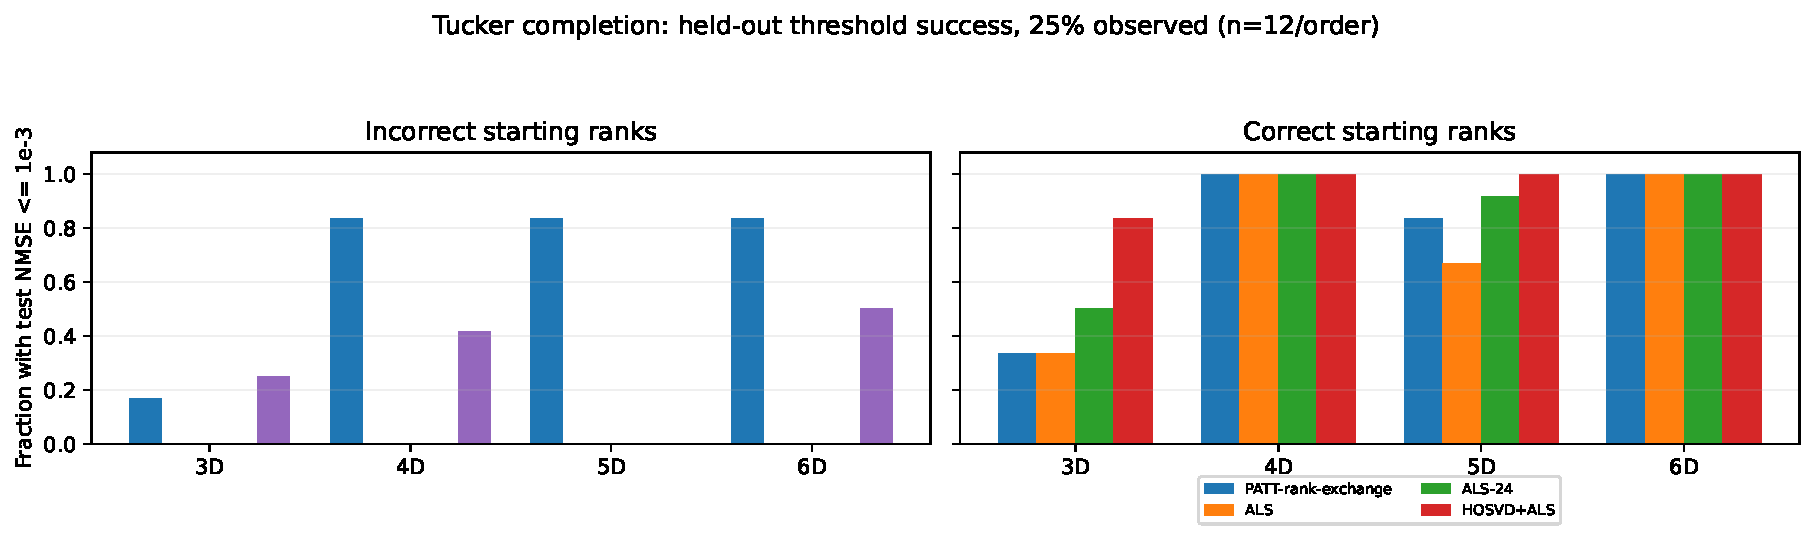
\includegraphics[width=.96\linewidth]{fig_success_by_order_and_rank_setup.pdf}
\caption{Accuracy-threshold attainment by tensor order for the wrong-rank and correct-rank setups. Counts are based on independent test entries, not a training-loss stopping rule.}\label{fig:success}
\end{figure}

The outcome also depends on the missingness pattern. Across the six MCAR seeds, PATT succeeds in $2/6$, $6/6$, $6/6$, and $6/6$ for orders three through six; across the six block-missing seeds it succeeds in $0/6$, $4/6$, $4/6$, and $4/6$. Structured missingness is therefore a clear weakness rather than a favorable test case. Figure~\ref{fig:paired} shows the paired PATT-versus-ALS test errors; it should be read jointly with the threshold counts rather than as a claim of superiority in every instance.

\begin{figure}[tbp]
\centering
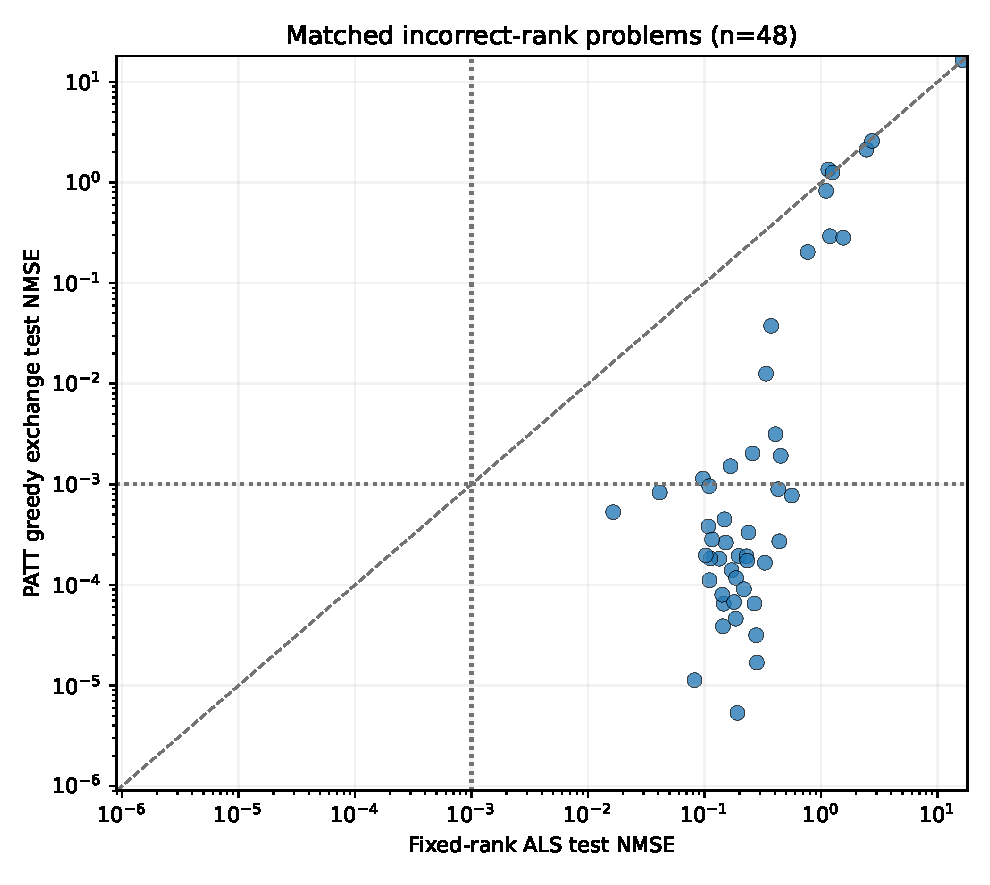
\includegraphics[width=.96\linewidth]{fig_paired_nmse_patt_vs_als.pdf}
\caption{Paired held-out NMSE for PATT rank exchange and fixed-rank Tucker-ALS under wrong rank allocation. The target threshold is $10^{-3}$.}\label{fig:paired}
\end{figure}

For the paired comparison with limited rank search, the exact McNemar test has $p=1.0$, $0.1797$, $0.001953$, and $0.2188$ for orders three through six, respectively. At only 12 paired trials per order, the results do not justify blanket statistical claims; in particular, only the fifth-order comparison is strongly separated in this exploratory calculation. The eight-candidate method occasionally succeeds where the exchange proposal fails, showing that rank allocation alone does not remove optimization sensitivity.


\subsection{Mechanism diagnostics, sampling geometry, and two misplaced ranks}\label{subsec:mechanism}

\begin{table}[tbp]
\caption{Actual rank-vector correction in the original paired 25\% wrong-rank study, derived directly from all 48 PATT trial records. A correct allocated rank vector is not a guarantee of accurate completion.}\label{tab:rankcorrect}
\centering\small
\begin{tabular}{lrrrr}
\toprule
Metric & Order 3 & Order 4 & Order 5 & Order 6\\
\midrule
Correct rank allocation & $7/12$ & $12/12$ & $11/12$ & $12/12$\\
Test NMSE $\le10^{-3}$ & $2/12$ & $10/12$ & $10/12$ & $10/12$\\
\bottomrule
\end{tabular}
\end{table}

In the original 48 wrong-rank PATT cases, the final \emph{allocated} ranks equal the true ranks in 42 trials, but test NMSE reaches $10^{-3}$ in only 32. This directly separates successful rank reallocation from complete tensor reconstruction. No stored factor histories are available for all of those trials, so donor-angle and feature-conditioning diagnostics cannot be retrospectively assigned to them. We instead evaluate these quantities in the separately generated, explicitly local mechanism test below.

To test the proposed \emph{mechanism} rather than only final threshold success, we ran 120 additional fourth-order one-swap trial configurations (20 random seeds per observation rate and mask type; seed values are reused across configurations). Shapes are $(8,9,7,7)$, true ranks $(2,2,2,2)$, and initial ranks $(3,1,2,2)$; the initial factor spaces satisfy the ideal one-swap containment model, but their \emph{cores are fitted from incomplete noisy entries}. Each instance uses noise standard deviation $0.002$ on observed entries after unit-RMS signal normalization. We recorded the donor and receiver angular errors, the largest and smallest nonzero normalized sampled feature Gram eigenvalues, the actual donor loss and receiver gain, and the two proposed certificates. Data used to generate the ground-truth factors are used only for evaluation, not receiver construction. The condition numbers are measured for the final candidate's sampled full-core design, not asserted upper bounds on every adaptive exchange subspace.

\begin{table}[tbp]
\caption{Direct greedy-mechanism measurements (20 independent trials per configuration). Entries ``old/new'' are frequencies of a \emph{positive} conservative certificate $\frac12(s_{ij}^2-\sigma_i^2)$ versus the mask-aware certificate~\eqref{eq:certgain}. All 120 mask-aware numerical certificates were below or equal to the measured training improvement; one-swap refitting alone did not attain held-out NMSE $10^{-3}$ in this test. Angular errors and Gram condition numbers are medians.}\label{tab:mechanism}
\centering\footnotesize
\begin{tabular}{ccrrrrr}
\toprule
Mask & $p$ & Donor $\sin\theta$ & Receiver $\sin\theta$ & $\kappa_{\rm Gram}$ & Old/new & Median NMSE\\
\midrule
MCAR & .10 & .160 & .304 & 8.51 & 12/20 & .0976\\
MCAR & .25 & .074 & .175 & 3.07 & 20/20 & .0250\\
MCAR & .40 & .059 & .114 & 2.20 & 20/20 & .0106\\
Block & .10 & .196 & .395 & 8.06 & 13/20 & .1148\\
Block & .25 & .078 & .242 & 3.87 & 20/20 & .0553\\
Block & .40 & .093 & .200 & 2.85 & 20/20 & .0402\\
\bottomrule
\end{tabular}
\end{table}

At $p=.10$, the mask-aware certificate is positive in all 40 trials, whereas the conservative certificate is positive in 25. The receiver angular error decreases substantially with increased MCAR sampling. The poorer block-mask errors are consistent with missing-data geometry being more harmful than rank misallocation alone. Because this is a deliberately initialized local mechanism test with one final core refit and \emph{no subsequent ALS sweeps}, it is not a general recovery success rate for the full algorithm. A random-search check of 60 eligible receiver directions per problem did not find a direction with larger gain than the spectral proposal; this is \emph{not} a certified ratio to the continuous optimum. The conservative random-mask sufficient bound~\eqref{eq:chernoff} does not certify the primary experimental training sizes; the observed Gram diagnostics provide empirical conditioning information rather than an unearned concentration guarantee.


For multiple-rank errors we distinguish a \emph{directly reachable two-transfer path} from a configuration with a budget barrier to that shortest path. Both experiments start at $(4,2,2,2)$ and target $(2,4,2,2)$, with $25\%$ observation, four MCAR seeds and four block-mask seeds. In the first, the shape $(15,9,10,9)$ gives starting, intermediate, and target parameter counts $148,146,136$, respectively. Both unit transfers are feasible. PATT executes two accepted rank exchanges in all eight trials and reaches NMSE $10^{-3}$ in $5/8$ (MCAR $4/4$, block $1/4$); the four fixed-rank short/long ALS and HOSVD-ALS controls all fail to reach the target. In the second, shape $(12,11,10,9)$ gives counts $140,143,138$: the direct intermediate allocation $(3,3,2,2)$ violates the initial budget. Nevertheless, a three-step feasible detour exists through $(4,3,1,2)$ and $(3,4,1,2)$, so the rank graph is \emph{not disconnected}. The implemented two-round greedy method makes no accepted exchange and achieves $0/8$ successes. Both are reported, since feasibility alone does not ensure a short or improving exchange path and neither result establishes arbitrary-initialization guarantees.

\begin{table}[tbp]
\caption{Two-misallocated-rank exploratory stress tests ($8$ trials each, with the identical start/target rank vectors but different mode dimensions). ``Transfers'' counts trials in which PATT accepted both rank exchanges. These cases are separate from the original benchmark.}\label{tab:twoswap}
\centering\small
\begin{tabular}{lrrr}
\toprule
Path & Budget (start/mid/target) & Two swaps & Success\\
\midrule
Reachable & $148,146,136$ & $8/8$ & $5/8$\\
Detour required & $140,143,138$ & $0/8$ & $0/8$\\
\bottomrule
\end{tabular}
\end{table}

The $h=2$ instance of Theorem~\ref{thm:hmode} passes an independent numerical check: each single-transfer candidate has zero full-data improvement, whereas the coordinated correction reconstructs the tensor with zero error. Separately, ten full-observation noiseless random one-swap trials recovered the ground-truth tensor with maximum squared NMSE $3.75\times10^{-31}$, confirming the exact theorem's algebra but not its robustness to missing observations.


\subsection{Pre-refitting certificates, longer horizons, and post-exchange refinement}\label{subsec:newcontrols}
Three focused controls distinguish the algebraic proposal from the actual accepted and refined iterate. They are \emph{additional} experiments, not part of the original paired trial counts. First, on 72 newly seeded order-four, one-misallocation problems (12 seeds for each of three sampling fractions and two mask patterns), the observed-only pre-refitting bound~\eqref{eq:prefitcert} was sound in all 72 trials and positive in all 72. The test generated the donor direction using the sampled fitted core, formed the raw-pruned residual and receiver SVD \emph{before} donor-core refitting, and compared the bound against the final exact core-fit improvement. This checks the certificate in a favorable constructed one-misallocation regime; it does not establish a universal screening rate, nor a runtime speedup of the unchanged implementation. For the \emph{same} 72 instances, we also evaluated the ideal-tensor-dependent sufficient quantities in Theorems~\ref{thm:stability} and~\ref{thm:localprogress} strictly as \emph{oracle diagnostics}. The incumbent sampled Gram distortion was below one in $60/72$ cases and the pruned Gram distortion was below one in $68/72$; nevertheless the full perturbation upper bound $\zeta$ exceeded the ideal receiver signal $s$ in every trial where both Gram conditions held. Consequently the theorem's strictly positive training margin could not be certified in \emph{any} of the 72 cases, despite all 72 having positive observed-data pre-refitting certificates. This is concrete evidence that the conservative a priori stability theorem does \emph{not} explain the success of these experiments. The implemented algorithm does not know the oracle quantities.

Second, repeating the same type of one-exchange initialization with the actual masked Tucker ALS refinement routine gave the following results on another 72 problems. With a single exchange and an exact core refit but \emph{no} subsequent ALS sweep, none met full-tensor NMSE $10^{-3}$. After three ALS sweeps, success was $31/36$ under MCAR sampling and $29/36$ with block masks; after ten sweeps it was $36/36$ in each mask group. This is direct empirical evidence that corrected allocations often still require continuous optimization. Neither a uniform row-coverage or regularity condition in Corollary~\ref{cor:alsstat} was certified from these trials.

\begin{table}[tbp]
\caption{Additional one-exchange mechanism tests (12 fresh seeds per mask and sampling fraction). The pre-refitting bound was valid and positive in all 72 instances. The right columns measure \emph{full-tensor} success after zero, three, or ten sweeps of the original Tucker ALS refinement routine; they are not new claims about the complete validation-gated PATT method.}\label{tab:refinecontrol}
\centering\small
\begin{tabular}{llrrrr}
\toprule
Mask & Train fraction & Positive certificate & 0 sweeps & 3 sweeps & 10 sweeps\\
\midrule
MCAR & $10\%$ & $12/12$ & $0/12$ & $7/12$ & $12/12$\\
MCAR & $25\%$ & $12/12$ & $0/12$ & $12/12$ & $12/12$\\
MCAR & $40\%$ & $12/12$ & $0/12$ & $12/12$ & $12/12$\\
Block & $10\%$ & $12/12$ & $0/12$ & $5/12$ & $12/12$\\
Block & $25\%$ & $12/12$ & $0/12$ & $12/12$ & $12/12$\\
Block & $40\%$ & $12/12$ & $0/12$ & $12/12$ & $12/12$\\
\bottomrule
\end{tabular}
\end{table}

Third, the budget-detour configuration of Table~\ref{tab:twoswap} was rerun on the same eight seeds with the allowed exchange horizon raised from two to three and then five. All runs still accepted \emph{zero} transfers and remained above the accuracy threshold. Increasing the horizon alone therefore does not resolve the initial greedy/validation stagnation. A separate full-data experiment verified Theorem~\ref{thm:hmode} for $h=2,3,4$: the best loss was $a^2/2$ after any $t<h$ transfers and zero after all $h$ coordinated transfers. We further implemented an explicit \emph{non-oracle limited block search} for a slightly enlarged version of the same constructed family: with $d=2h+2$ three-dimensional modes, the $h$ redundant donor modes are identified by their surplus allocated ranks, but the correct $h$ receiver modes are \emph{not supplied} to the search. For each feasible receiver subset of size $h$, it first prunes all $h$ donor directions, contracts the observed full residual against the nonreceiver factors, extracts the leading left singular vector in every proposed receiving mode, appends the $h$ new directions simultaneously, and compares the final exactly fitted core losses. Wrong subsets have zero projected missing-component signal in this construction; the correct subset is recognized without knowing its indices. The number of candidate receiver subsets grows as $\binom{h+2}{h}$ here, and general donor--receiver subset enumeration can require $O\bigl(\binom{d}{h}^2\bigr)$ configurations. This is a \emph{fully observed constructive control}, not a new general-purpose masked PATT baseline. All nine amplitude/order combinations reached zero loss, as detailed below. Increasing the number of allowed greedy rounds was \emph{not} used as a proxy for lookahead.



\begin{table}[tbp]
\caption{Implemented full-observation $h$-way block-subset search on the constructed coupled-deficiency family. The receiver modes were selected by residual contractions, not supplied as oracle input. These are small deterministic controls, not matched incomplete-tensor benchmarks.}\label{tab:blocktoy}
\centering\small
\begin{tabular}{rrrrr}
\toprule
Coupled modes $h$ & Order $d$ & Feasible subsets & Recovered & Final loss\\
\midrule
2 & 6 & 6 & $3/3$ & 0\\
3 & 8 & 10 & $3/3$ & 0\\
4 & 10 & 15 & $3/3$ & 0\\
\bottomrule
\end{tabular}
\end{table}

\paragraph{Algorithm-aligned receiver and ALS audits.}
On 72 further fresh observed-data instances (12 seeds per combination of three observation fractions and two mask classes), we applied exactly the post-pruning residual-SVD direction used in Algorithm~\ref{alg:patt}. The bound~\eqref{eq:postdonorcert} was positive and valid in 72/72 cases, as was the raw-to-refit bridge bound~\eqref{eq:bridgecert}; all 72 proposals lowered the \emph{training} objective. These are separate from the original PATT success counts and do not test validation acceptance. In 36 further independent near-true, correct-rank synthetic starts, the actual factor-row ALS routine satisfied the row-level identity~\eqref{eq:alsrowgain} and the sweep-level \emph{inequality}~\eqref{eq:alssweepactual} in 36/36; all rows happened to meet its minimum observation-count condition, and the maximum measured QR gauge-objective deviation was less than $10^{-15}$. These tests verify the new identities numerically, not full reconstruction success or asymptotic convergence.

For a more targeted \emph{oracle-only} receiver stability diagnostic, we computed the full-data ideal rank-one residual direction using synthetic ground truth, then separated actual residual perturbations parallel and orthogonal to that direction. The margin $A_u>D_u$ in Theorem~\ref{thm:offsig} held in 70/72 cases, and the angular bound was verified in \emph{all 70 applicable cases}. The other two instances do not satisfy the theorem hypothesis: assigning them $90^\circ$ is a descriptive fallback, \emph{not} a verification of the conditional theorem. Across the 70 applicable cases, the median predicted angle upper bound was $19.17^\circ$ (interquartile interval $9.75^\circ$--$30.31^\circ$), compared with a median observed angle of $16.92^\circ$. The previous \emph{sum-of-worst-case} stability bound from Theorem~\ref{thm:stability} still certified none of the original diagnostic cases. These two results are not contradictory: the targeted analysis uses \emph{realized oracle perturbations}, whereas the prior theorem propagates multiple conservative a priori bounds. Neither result supplies a high-probability sampling guarantee for adaptively learned factors.

\begin{table}[tbp]
\caption{New algorithm-aligned numerical checks (disjoint synthetic seeds). ``Positive'' refers to observed-data \emph{training}-loss certificates, not validation acceptance; targeted stability uses true factors for evaluation only.}\label{tab:review4audit}
\centering\small
\begin{tabular}{p{0.67\linewidth}r}
\toprule
Test & Verified/trials\\
\midrule
Actual post-pruning receiver gain certificate: valid and positive & 72/72\\
Raw--refitted contraction bridge: valid and positive & 72/72\\
Implemented row-level descent identity and sweep inequality & 36/36\\
Targeted oracle spectral margin $A_u>D_u$ & 70/72\\
Targeted oracle angular bound, applicable cases only & 70/70\\
Spectral condition not met, theorem inapplicable & 2/72\\
\bottomrule
\end{tabular}
\end{table}
\subsection{Algorithm-level screening, stationarity, and basin diagnostics}\label{subsec:review5}
Four focused controls are presented below. The targeted-progress audit reuses the 72 oracle-stability configurations; the stationarity, certified-priority, and basin tests use independent new seeds. None changes the primary paired results in Table~\ref{tab:wrong}.

\paragraph{Targeted progress and angular applicability.}
For the same 72 fresh masked cases used in the oracle angle audit, we computed $A_u$, $D_u$, the actual donor-refit loss $\ell_i$, and the selected receiver's residualized sampled feature-Gram norm $\Lambda$. The new lower bound~\eqref{eq:targetgain} was below the directly fitted training gain and positive in 72/72 cases. The strict angular condition $A_u>D_u$ applied in 70/72; its angular inequality held in 70/70 eligible trials, while the remaining two are recorded solely as inapplicable. The more conservative angle-to-gain lower bound~\eqref{eq:anglegain} was positive in 66/72 cases. All these diagnostics use the ideal direction $u$ for post hoc evaluation and cannot certify an unknown tensor from sampled data alone.

\paragraph{Skipped rows and actual stationarity.}
We repeated one full executed ALS sweep on 48 newly seeded fourth-order masked problems, 12 at each training fraction $0.002$, $0.005$, $0.01$, and $0.10$. The allocated rank was $(2,2,2,2)$, and there were 31 physical factor rows. We measured minimum positive row-Gram eigenvalues, the number of skipped rows, the gauge-horizontal factor gradient on those rows, and the current core-gradient norm. Table~\ref{tab:skiprows} reports the median measurements after one full sweep. Very sparse masks can yield an almost zero training gradient despite a highly underdetermined completion problem: a small training stationarity residual is not an unseen-entry accuracy certificate.
\begin{table}[tbp]
\caption{Observed one-sweep coverage and stationarity diagnostics (12 seeds per fraction). Reported minima are over executed rows; zero skipped-row gradient when no rows are skipped is structural. All gradients are evaluated at the \emph{same final sweep boundary}, not conflated with the earlier row-update gradients in~\eqref{eq:alsrowgain}.}\label{tab:skiprows}
\centering\small
\begin{tabular}{rrrr}
\toprule
Training fraction & Skipped rows & Min. row Gram eig. & $\mathfrak R_{\rm skip}$\\
\midrule
0.002 & 24 & $1.1\times10^{-5}$ & $<10^{-6}$\\
0.005 & 9 & $3.0\times10^{-6}$ & $1.6\times10^{-5}$\\
0.010 & 2 & $2.3\times10^{-5}$ & $6.4\times10^{-5}$\\
0.100 & 0 & $9.9\times10^{-2}$ & $0$\\
\bottomrule
\end{tabular}
\end{table}

\paragraph{Certified-priority variant and computational savings.}
We implemented a \emph{separate} certified-priority variant: after the shared donor-refit and receiver-SVD calculations, candidates are ordered by the observable lower bound~\eqref{eq:postdonorcert}; the variant performs expanded-core fitting and two refinement sweeps in this order, and stops at the first validation-improving candidate that does not increase training loss. A negative bound is \emph{not} used to discard any candidate. This early-accept policy differs from Algorithm~\ref{alg:patt}, which expands all candidates, shortlists the four best training fits, and chooses minimum validation loss after refinement. Therefore the two variants are paired as different algorithms rather than claimed mathematically equivalent. On 24 newly seeded, wrong-rank experiments (12 each of orders four and five, with $25\%$ and $40\%$ observations), both variants reached the target in 23/24 trials. Table~\ref{tab:priority} reports expanded-core fits and measured end-to-end one-round wall time. These favorable single-misallocation results do not establish the same speedup for difficult masks, multiple rank errors, or general benchmarks.
\begin{table}[tbp]
\caption{Measured comparison with a newly implemented certified-priority variant (12 paired cases per order). Runtimes include common donor fits, receiver-score generation, candidate solves and short refinement; experiments use a single BLAS thread.}\label{tab:priority}
\centering\small
\begin{tabular}{clrrr}
\toprule
Order & Method & Expanded fits & Median time (s) & Success\\
\midrule
4 & Original shortlist & 12 & 0.133 & 11/12\\
4 & Certified priority & 1 & 0.044 & 11/12\\
5 & Original shortlist & 20 & 0.979 & 12/12\\
5 & Certified priority & 1 & 0.303 & 12/12\\
\bottomrule
\end{tabular}
\end{table}

\paragraph{Actual post-exchange refinement and basin diagnostic.}
We produced 36 independent fourth-order one-swap instances with 2\%, 10\%, or 25\% observed entries, equally split between MCAR and rectangular-block masks. Donor deletion and receiver SVD used only the training mask; true subspaces were used solely to compute post-exchange principal-angle diagnostics. We then ran ten \emph{actual} masked Tucker ALS sweeps without additional exchanges. The ten-sweep held-out NMSE threshold was met in $0/12$ cases at 2\% training observations, $12/12$ at 10\%, and $12/12$ at 25\%. The corresponding median initial maximum principal-angle sines were $0.783$, $0.410$, and $0.263$ (rounded). These results support the need to analyze local subspace quality after reallocation; they do \emph{not} verify the uniform Jacobian-contraction assumption in Theorem~\ref{thm:basin}, nor do they retroactively explain each of the original ten rank-corrected failures, for which per-iteration factors were not saved.

\subsection{Correct-rank controls and limits of the claim}\label{subsec:correct}
Table~\ref{tab:correct} repeats the paired study with correct initial Tucker ranks. Ordinary ALS and HOSVD-based initialization are then competitive or better. In particular, HOSVD $+$ ALS reaches $10/12$ order-three successes while PATT reaches $4/12$, and both attain $12/12$ on the order-four and order-six controls. This is central evidence for the intended contribution: greedy rank reallocation is useful mainly when the allocated mode dimensions are wrong.

\begin{table}[tbp]
\caption{Held-out NMSE $\le10^{-3}$ under \emph{correct} initial Tucker ranks (12 trials per order).}\label{tab:correct}
\centering\small
\begin{tabular}{lcccc}
\toprule
Method & Order 3 & Order 4 & Order 5 & Order 6\\
\midrule
PATT rank exchange & $4/12$ & $12/12$ & $10/12$ & $12/12$\\
Tucker-ALS & $4/12$ & $12/12$ & $8/12$ & $12/12$\\
Tucker-ALS (24 sweeps) & $6/12$ & $12/12$ & $11/12$ & $12/12$\\
HOSVD $+$ Tucker-ALS & $10/12$ & $12/12$ & $12/12$ & $12/12$\\
\bottomrule
\end{tabular}
\end{table}

A separate ablation tested same-rank direction replacement and spectral-guided restart candidates. The finite-replacement variant did not add threshold successes consistently and often increased runtime. Rather than attributing the observed gains to an unvalidated replacement mechanism, we make the rank-exchange prototype the main evaluated algorithm. Full joint subspace replacement is a possible extension, not a supported result of this paper.

\subsection{Published-algorithm ports and real-data control}\label{subsec:supplement}
For additional context we ran source-guided Python translations of TRAM \cite{GaoPengYuan2025} and TMac \cite{XuHaoYinSu2015} on corresponding small problems. These translations are documented, but numerical equality with the authors' MATLAB/MEX execution has not been established. TRAM's port addresses third-order Tucker optimization; TMac optimizes factorizations of mode matricizations, which is not the same objective as \eqref{eq:objective}. The image-specific ARE wrapper \cite{MiHeLiLiu2026} required corrections to avoid using held-out image information and is not treated as a general-order Tucker baseline. Consequently, we treat these runs as supplementary software comparisons, not original-code benchmarks that establish method-level superiority.

To test a failure mode outside the exact synthetic Tucker model, we assembled a fourth-order tensor of size $12\times12\times8\times8$ from 144 handwritten digit images in the public scikit-learn digits dataset. There are 12 trials per method across 25\% and 40\% observation fractions, MCAR and block masks, and three seeds per condition. No evaluated method attained $10^{-3}$ at the deliberately small imposed rank budget. Table~\ref{tab:digits} records this negative control; the result is consistent with representational mismatch and is not evidence of impossibility for larger ranks.

\begin{table}[tbp]
\caption{Real-digit tensor control under a restricted Tucker budget (12 trials per method). All methods fail to reach NMSE $10^{-3}$.}\label{tab:digits}
\centering\small
\begin{tabular}{lrr}
\toprule
Method & Successes & Median test NMSE\\
\midrule
PATT rank exchange & $0/12$ & $0.3671$\\
Tucker-ALS & $0/12$ & $0.3771$\\
Tucker-ALS (longer) & $0/12$ & $0.3853$\\
Imputation-HOOI & $0/12$ & $0.3741$\\
Tucker rank search ($\le8$) & $0/12$ & $0.3538$\\
\bottomrule
\end{tabular}
\end{table}

\subsection{Reproducibility and limitations}\label{subsec:limitations}
The accompanying reproducibility package contains full per-run data, independent-seed records, Python solver implementations, validation/test splits and figure-generation scripts. Its primary paired dataset comprises 432 solver records, with another 528 records from the source-guided TRAM/TMac ports and 60 real-data solver records. A run with test NMSE below $10^{-3}$ is counted as successful regardless of additional numerical accuracy; the earliest recorded \emph{validation} threshold crossing is not mislabeled as a test-time crossing. All median runtimes in Table~\ref{tab:medians} refer to the entire executed fit.

The study has five limitations. First, its main comparison uses synthetic tensors of modest size and intentional rank misallocation. Second, baseline implementations are locally written Python code; original external MATLAB releases were inspected but not run for numerical parity. Third, acceptance depends on validation error, so the training-descent theorem does not imply held-out monotonicity. Fourth, neither large-scale peak-memory advantages nor multicore parallel speedups have been established by this study. Fifth, even increasing the two-misallocation budget-detour horizon to five exchange rounds yields no accepted move in the evaluated cases; the separately implemented full-data block-subset control, pre-refitting prioritization, and fresh-batch validation are not performance-validated as integrated variants on the primary masked benchmark. The new 72-case refinement study uses a controlled one-exchange start and does not certify global ALS convergence. These restrictions delimit the scope of the conclusions.


\section{Conclusion}\label{sec:conclusion}
This study isolates a practical corrective operation for Tucker completion: a budget-feasible donor--receiver rank transfer followed by core refitting and local factor optimization. The principal analysis now compares donor SVD deletion with the best donor-only truncation under sampled conditioning, provides a mask-aware bound on actual exchange gain, and proves quantitative \emph{joint} donor and receiver stability. In a locally identifiable one-misallocation regime, an a priori inequality gives a positive training-gain condition for an exact core-refitted proposal, but its conservative perturbation bounds certify none of the new diagnostic trials and it does not ensure acceptance by the evaluated validation gate. The general $h$-mode counterexample shows that a strictly improving one-swap algorithm can fail even when the correct allocation is connected by budget-feasible transfers; a coordinated $h$-mode spectral proposal can overcome the constructed obstruction but is not part of the benchmarked algorithm. New mechanism diagnostics verify the algebraic certificates and show substantial but imperfect subspace recovery, while the two-misallocation tests distinguish successful sequential correction from a shortest-path budget barrier and observed greedy stagnation. The original paired experiments demonstrate useful rank-correction behavior primarily on particular fourth- through sixth-order synthetic instances, not universal Tucker model superiority. The newly derived pre-refitting certificate offers an observable training-gain check before candidate-specific core solves, while the separate post-exchange tests show why continuous ALS refinement is needed even after correct rank allocation; the new row-wise descent theorem proves a guarantee for those implemented updates but not unconditional basin entry. The original validation-gated shortlist can still reject a certified proposal, and the probabilistic sampling conditions are not certified for the main benchmark. An independently evaluated certified-priority screening variant reduces candidate core solves in the favorable one-misallocation regime without changing threshold success, but is not the original shortlist implementation. A sharper oracle off-signal bound produces positive proposal-level gains even when the conservative bulk perturbation condition fails; neither gives an unconditional validation-acceptance or basin-entry guarantee. New skipped-row and post-exchange diagnostics distinguish training stationarity from reconstruction quality. Reliable fresh-batch validation, uniform adaptive-mask sampling control, and unrestricted block donor--receiver search remain open.


\section*{Data and code availability}
The per-run numerical results, dataset-generation scripts, and independent Python implementations used here are provided in the supplementary experimental package accompanying this manuscript. No authors' official MATLAB/MEX baseline outputs are claimed.

\begin{thebibliography}{99}
\bibitem{KoldaBader2009}
T. G. Kolda, B. W. Bader, Tensor decompositions and applications, SIAM Review 51 (3) (2009) 455--500. \url{https://doi.org/10.1137/07070111X}.
\bibitem{DeLathauwer2000svd}
L. De Lathauwer, B. De Moor, J. Vandewalle, A multilinear singular value decomposition, SIAM J. Matrix Anal. Appl. 21 (4) (2000) 1253--1278. \url{https://doi.org/10.1137/S0895479896305696}.
\bibitem{DeLathauwer2000best}
L. De Lathauwer, B. De Moor, J. Vandewalle, On the best rank-1 and rank-$(R_1,R_2,\ldots,R_N)$ approximation of higher-order tensors, SIAM J. Matrix Anal. Appl. 21 (4) (2000) 1324--1342. \url{https://doi.org/10.1137/S0895479898346995}.
\bibitem{KasaiMishra2016}
H. Kasai, B. Mishra, Low-rank tensor completion: a Riemannian manifold preconditioning approach, in: Proc. 33rd Int. Conf. Machine Learning, PMLR 48 (2016) 1012--1021. \url{https://proceedings.mlr.press/v48/kasai16.html}.
\bibitem{XuHaoYinSu2015}
Y. Xu, R. Hao, W. Yin, Z. Su, Parallel matrix factorization for low-rank tensor completion, Inverse Problems and Imaging 9 (2) (2015) 601--624. \url{https://doi.org/10.3934/ipi.2015.9.601}.
\bibitem{LiuShiLiao2023}
S. Liu, X. Shi, Q. Liao, Rank-adaptive tensor completion based on Tucker decomposition, Entropy 25 (2) (2023) 225. \url{https://doi.org/10.3390/e25020225}.
\bibitem{GaoPengYuan2025}
B. Gao, R. Peng, Y.-x. Yuan, Low-rank optimization on Tucker tensor varieties, Mathematical Programming 214 (1) (2025) 357--407. \url{https://doi.org/10.1007/s10107-024-02186-w}.
\bibitem{MiHeLiLiu2026}
C. Mi, J. He, A. Li, X. Liu, Plug-and-play adaptive rank estimation for low-rank tensor completion, Signal Processing 242 (2026) 110421. \url{https://doi.org/10.1016/j.sigpro.2025.110421}.
\bibitem{LiuMusialskiWonkaYe2013}
J. Liu, P. Musialski, P. Wonka, J. Ye, Tensor completion for estimating missing values in visual data, IEEE Trans. Pattern Anal. Mach. Intell. 35 (1) (2013) 208--220. \url{https://doi.org/10.1109/TPAMI.2012.39}.
\bibitem{Tropp2012}
J. A. Tropp, User-friendly tail bounds for sums of random matrices, Foundations of Computational Mathematics 12 (2012) 389--434. \url{https://doi.org/10.1007/s10208-011-9099-z}.
\end{thebibliography}
\end{document}
